% presentation
%\documentclass[compress,draft]{beamer}
\documentclass[compress,aspectratio=1610,fleqn]{beamer}
%\documentclass[compress,aspectratio=1610,handout]{beamer}

%\includeonlyframes{current}


\usepackage{../mtex,fancyvrb,booktabs,multirow,makecell}
\usepackage{tikz,pgfplots,multicol}
\usetikzlibrary{shapes,calc,angles,quotes,external}
\usepackage{tasks,nccmath}
\settasks{counter-format=tsk[a]),label-width=1em,before-skip=0.5em}
\RenewTasks{enumerate}[\item]

\makeatletter
\newcommand*{\overlaynumber}{\number\beamer@slideinframe}
\tikzset{
  beamer externalizing/.style={%
    execute at end picture={%
      \tikzifexternalizing{%
        \ifbeamer@anotherslide
        \pgfexternalstorecommand{\string\global\string\beamer@anotherslidetrue}%
        \fi
      }{}%
    }%
  },
  external/optimize=false
}
\let\orig@tikzsetnextfilename=\tikzsetnextfilename
\renewcommand\tikzsetnextfilename[1]{\orig@tikzsetnextfilename{#1-\overlaynumber}}
\DeclareMathOperator*{\argmin}{argmin}
\makeatother

\tikzset{every picture/.style={beamer externalizing}}
\tikzexternalize

\newcommand{\rz}{\ensuremath \mathbb{R}}   %reelle Zahlen


%\usepackage{subfigure}
\usepackage[labelformat=empty]{subcaption}
\captionsetup{compatibility=false}
%\usepackage[inline]{enumitem}
\newcommand\paraitem{%
  \;
  \makebox[\labelwidth][r]{%
    \makelabel{%
      \usebeamertemplate{itemize \beameritemnestingprefix item}}}\hskip\labelsep}


\newcommand{\SO}{\mathrm{SO}(3)}
\newcommand{\rot}[1]{\mathbf{#1}}
\newcommand{\ds}{\displaystyle}
\newcommand{\R}{\mathbb R}
\renewcommand{\S}{\mathbb S}
\newcommand{\conj}[1]{\overline{#1}}
\newcommand{\norm}[1]{\lVert #1\rVert}
\newcommand{\abs}[1]{\lvert #1\rvert}
\newcommand{\laplace}{\triangle}

\DeclareMathOperator{\argmax}{argmax}


\newcommand{\mytriangle}[1]{\tikz{\node[draw=#1,fill=#1,isosceles
triangle,isosceles triangle stretches,shape border rotate=90,minimum
width=0.2cm,minimum height=0.2cm,inner sep=0pt] at (0,0) {};}}

\usetikzlibrary{fit}
% \tikzset{%
%   highlight/.style={rectangle,rounded corners,fill=red!15,draw,
%     fill opacity=0.5,thick,inner sep=0pt}
%   }
\tikzset{%
  highlight/.style={rectangle,rounded corners,draw,red,
    fill opacity=0.5,thick,inner sep=0pt}
}
% see https://tex.stackexchange.com/questions/40028/highlight-elements-in-the-matrix

\newcommand{\tikzmark}[2]{\tikz[overlay,remember picture,
  baseline=(#1.base)] \node (#1) {#2};}
%
\newcommand{\Highlight}[1][submatrix]{%
    \tikz[overlay,remember picture]{
    \node[highlight,fit=(left.north west) (right.south east)] (#1) {};}
}


\renewcommand{\arraystretch}{1.4}

\author{Ralf Hielscher}

\title{Plasticity}

\institute{Faculty of Mathematics and Computer Science,\\
	TU Bergakademie Freiberg, Germany}

\date{MTEX Workshop 2024}


\begin{document}

\begin{frame}
  \maketitle{}
\end{frame}


\begin{frame}[fragile]
  \frametitle{The Velocity Gradient Tensor}%

  \begin{overlayarea}{\textwidth}{7.5cm}
    describes the local rate of deformation
    \vspace{-0.2cm}
\begin{lstlisting}[style=input]
L = velocityGradientTensor.uniaxial(vector3d.Z)
\end{lstlisting}
    \begin{onlyenv}<1|handout:0>
      \vspace{-0.3cm}
\begin{lstlisting}[style=output]
L = /+velocityGradientTensor+/ (xyz)
  rank: 2 (3 x 3)

 -0.5    0    0
    0 -0.5    0
    0    0    1
\end{lstlisting}
    \end{onlyenv}
%
    \pause
%
\begin{lstlisting}[style=input]
d_exp = vector3d.Y; d_compr = vector3d.X;
L = velocityGradientTensor.pureShear(d_exp,d_compr)
\end{lstlisting}
    \begin{onlyenv}<2|handout:0>
      \vspace{-0.3cm}
\begin{lstlisting}[style=output]
L = /+velocityGradientTensor+/ (xyz)
  rank: 2 (3 x 3)

  -2  0  0
   0  2  0
   0  0  0
\end{lstlisting}
    \end{onlyenv}
    %
    \pause
%
\begin{lstlisting}[style=input]
d = vector3d.Y; n = vector3d.X;
L = velocityGradientTensor.simpleShear(d,n)
\end{lstlisting}
    \begin{onlyenv}<3|handout:0>
      \vspace{-0.3cm}
\begin{lstlisting}[style=output]
L = /+velocityGradientTensor+/ (xyz)
  rank: 2 (3 x 3)

 0 0 0
 2 0 0
 0 0 0
\end{lstlisting}
    \end{onlyenv}
    %
    \pause
%
\begin{lstlisting}[style=input]
rot = rotation.byAxisAngle(vector3d.Z, 10*degree)
L = velocityGradientTensor.spin(rot)
\end{lstlisting}
    \begin{onlyenv}<4|handout:0>
      \vspace{-0.3cm}
\begin{lstlisting}[style=output]
L = /+spinTensor+/ (xyz)
  rank: 2 (3 x 3)

 *10^-2
       0 -17.453       0
  17.453       0       0
       0       0       0
\end{lstlisting}
    \end{onlyenv}
  \end{overlayarea}
\end{frame}


\begin{frame}[fragile]
  \frametitle{Decomposition of the Velocity Gradient Tensor}

  \begin{overlayarea}{\textwidth}{7.5cm}
    The deformation gradient tensor can be decomposed into a sum of a
    symmetric and an antisymmetric tensor
              \vspace{-0.2cm}
\begin{lstlisting}[style=input]
W = L.antiSym
D = L.sym
\end{lstlisting}
    \begin{onlyenv}<1|handout:0>
          \vspace{-0.3cm}
\begin{lstlisting}[style=output]
W = /+spinTensor+/ (xyz)
  rank: 2 (3 x 3)

   0  -1  0
   1   0  0
   0   0  0

D = /+strainRateTensor+/ (xyz)
  rank: 2 (3 x 3)

  0  1  0
  1  0  0
  0  0  0
\end{lstlisting}
    \end{onlyenv}

    \medskip

    \begin{onlyenv}<2->
      the antisymmetric portion models the spin
          \vspace{-0.2cm}
\begin{lstlisting}[style=input]
rotation(W)
\end{lstlisting}
    \end{onlyenv}
    \begin{onlyenv}<2>
      \vspace{-0.3cm}
\begin{lstlisting}[style=output]
ans = /+rotation+/
  size: 1 x 1

  Bunge Euler angles in degree
  phi1   Phi    phi2    Inv.
  57.3     0       0       0
\end{lstlisting}
    \end{onlyenv}
  \end{overlayarea}
\end{frame}


\begin{frame}[fragile,fragile,fragile]
  \frametitle{The Deformation Gradient Tensor $\mathbf F$}

  \begin{overlayarea}{\textwidth}{7.5cm}
    describes the local deformation in continuum mechanics and satisfies
    \begin{equation*}
      \dot{\mathbf F}(t) = \mathbf L(t) \, \mathbf F(t)
    \end{equation*}

    \pause

    In case of constant deformation $\mathbf L(t) = \mathbf L$ we obtain
  \begin{equation*}
    \mathbf F(t) = \exp(t \cdot \mathbf L)
  \end{equation*}
  \pause
  \vspace{-1cm}
\begin{lstlisting}[style=input]
F = expm(L * t)
\end{lstlisting}
  \begin{onlyenv}<3|handout:0>
    \vspace{-0.3cm}
\begin{lstlisting}[style=output]
F = /+deformationGradientTensor+/ (xyz)
  rank: 2 (3 x 3)

 1 0 0
 2 1 0
 0 0 1
\end{lstlisting}
  \end{onlyenv}

  \pause
  \medskip
  %
  In the case of time dependent deformation we have
  \begin{equation*}
    \mathbf F(t) = \exp\left( \int_{0}^{t} \mathbf L(\tau) \, \mathrm d \tau \,\right)
  \end{equation*}
  %this translates into MTEX via
  \vspace{-0.5cm}
\begin{lstlisting}[style=input]
tau = linspace(0,t); d_tau = tau(2)-tau(1);
L_tau = (t-tau) .* L
F = expm(cumsum(L_tau * d_tau))
\end{lstlisting}



  % \vspace {-0.2cm}
  % \begin{lstlisting}[style=input]
  % d = vector3d.Y n = vector3d.X F =
% deformationGradientTensor.simpleShear(d,n)
% \end{lstlisting}
% \begin{onlyenv}<1> \vspace{-0.2cm}
% \begin{lstlisting}[style=output]
% F = /+deformationGradientTensor+/ (xyz)
%   rank: 2 (3 x 3)

%  1 0 0
%  2 1 0
%  0 0 1
% \end{lstlisting}
% \end{onlyenv}

% \medskip \pause



% \begin{lstlisting}[style=input]
% [R,U,V] = polar(L)
% \end{lstlisting}
% \begin{overlayarea}{\textwidth}{8cm}

% \end{overlayarea}

\end{overlayarea}
\end{frame}


\begin{frame}[fragile]
  \frametitle{Decomposition of the Deformation Gradient Tensor}

  \begin{columns}
    \begin{column}{0.55\textwidth}
      \begin{overlayarea}{\textwidth}{0.85\textheight}
        The deformation gradient tensor $\mathbf F$ can be decomposed into a
        rotational part $\mathbf R$, a right stretch tensor $\mathbf U$ and a
        left stretch tensor $\mathbf V$ such that
        \begin{equation*}
          \mathbf F = \mathbf R \mathbf U = \mathbf V \mathbf R
        \end{equation*}
\vspace{-0.8cm}
\begin{lstlisting}[style=input]
[R,V,U] = polar(F)
\end{lstlisting}
        \begin{onlyenv}<1|handout:0>
          \vspace{-0.3cm}
\begin{lstlisting}[style=output]
R = /+tensor+/ (xyz)
  rank: 2 (3 x 3)

  0.7071 -0.7071       0
  0.7071  0.7071       0
       0       0       1

U = /+tensor+/ (xyz)
  rank: 2 (3 x 3)

 2.1213 0.7071      0
 0.7071 0.7071      0
      0      0      1
\end{lstlisting}
        \end{onlyenv}

        \medskip
  \pause

The polar decomposition is closely related to the singular value decomposition
of of $\mathbf F$
\begin{lstlisting}[style=input]
[v,s,u] = svd(expm(L .* tau))
\end{lstlisting}
%
\pause
%
\vspace{-0.2cm}
\begin{lstlisting}[style=input]
a = s(1); b = s(3);
plotEllipse([0,0],a,b,u(1).rho)
\end{lstlisting}
%
\pause
%
\vspace{-0.2cm}
\begin{lstlisting}[style=input]
plotEllipse([0,0],a,b,v(1).rho)
\end{lstlisting}
\end{overlayarea}
\end{column}
\begin{column}{0.42\textwidth}
  \begin{overlayarea}{\textwidth}{0.85\textheight}
    \begin{onlyenv}<3->
      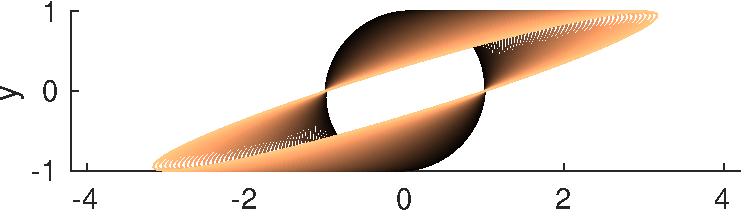
\includegraphics[width=\textwidth]{pic/strainEllipseRight.pdf}
    \end{onlyenv}
    \begin{onlyenv}<4>
      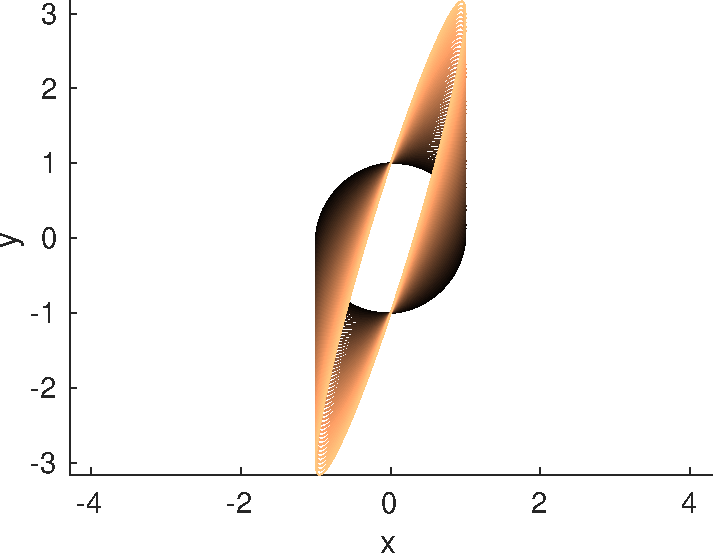
\includegraphics[width=\textwidth]{pic/strainEllipseLeft.pdf}
    \end{onlyenv}
  \end{overlayarea}


\end{column}
\end{columns}

\end{frame}


\begin{frame}[fragile]
%
  \frametitle{Strain Tensors}
          \vspace{-0.5cm}
     \begin{columns}
      \begin{column}{0.55\textwidth}
        \begin{overlayarea}{\textwidth}{7.5cm}
          right Cauchy-Green stretch tensor
          $\mathbf C = \mathbf U^2 = \mathbf F' \mathbf F$ \vspace{-0.2cm}
\begin{lstlisting}[style=input]
C = F` .* F
\end{lstlisting}

          \vspace{0.2cm}

          \begin{onlyenv}<2-> left Cauchy-Green stretch tensor
            $\mathbf B = \mathbf V^2 = \mathbf F \mathbf F'$ \vspace{-0.2cm}
\begin{lstlisting}[style=input]
B = F .* F`
\end{lstlisting}
          \end{onlyenv}

          \vspace{0.2cm}

          \begin{onlyenv}<3-> Green-Lagrange strain tensor \vspace{-0.2cm}
\begin{lstlisting}[style=input]
E = (C - tensor.eye)./2
\end{lstlisting}
          \end{onlyenv}

          \vspace{0.2cm}

          \begin{onlyenv}<4-> Almansi strain tensor \vspace{-0.2cm}
\begin{lstlisting}[style=input]
e = (tensor.eye - inv(B))./2
\end{lstlisting}
          \end{onlyenv}

          \vspace{0.2cm}

          \begin{onlyenv}<5-> engineering strain \vspace{-0.2cm}
\begin{lstlisting}[style=input]
eps = F.sym - tensor.eye
\end{lstlisting}
          \end{onlyenv}

          \vspace{0.2cm}

          \begin{onlyenv}<6-> true, logarithmic or Hencky strain tensor
            \vspace{-0.2cm}
\begin{lstlisting}[style=input]
H = logm(U)
\end{lstlisting}
          \end{onlyenv}
        \end{overlayarea}

  \end{column}
      \begin{column}{0.4\textwidth}
  \begin{overlayarea}{\textwidth}{\textheight}
        \begin{onlyenv}<1|handout:0>
\begin{lstlisting}[style=output]
C = /+tensor+/ (xyz)
  rank: 2 (3 x 3)

      1 0.0524      0
 0.0524 1.0027      0
      0      0      1
\end{lstlisting}
        \end{onlyenv}
        \begin{onlyenv}<2|handout:0>
\begin{lstlisting}[style=output]
B = /+tensor+/ (xyz)
  rank: 2 (3 x 3)

 1.0027 0.0524      0
 0.0524      1      0
      0      0      1
\end{lstlisting}
        \end{onlyenv}
        \begin{onlyenv}<3|handout:0>
\begin{lstlisting}[style=output]
E = /+tensor+/ (xyz)
  rank: 2 (3 x 3)

 *10^-3
      0 26.204      0
 26.204  1.373      0
      0      0      0
\end{lstlisting}
        \end{onlyenv}
        \begin{onlyenv}<4|handout:0>
\begin{lstlisting}[style=output]
e = /+tensor+/ (xyz)
  rank: 2 (3 x 3)

 *10^-3
      0 26.204      0
 26.204 -1.373      0
      0      0      0
\end{lstlisting}
        \end{onlyenv}
        \begin{onlyenv}<5|handout:0>
\begin{lstlisting}[style=output]
eps = /+tensor+/ (xyz)
  rank: 2 (3 x 3)

 *10^-3
      0 26.204      0
 26.204      0      0
      0      0      0
\end{lstlisting}
        \end{onlyenv}
        \begin{onlyenv}<6->
\begin{lstlisting}[style=output]
H = /+tensor+/ (xyz)
  rank: 2 (3 x 3)

 *10^-3
 -0.686 26.192      0
 26.192  0.686      0
      0      0      0
\end{lstlisting}
        \end{onlyenv}

        \bigskip

        \begin{onlyenv}<7>
          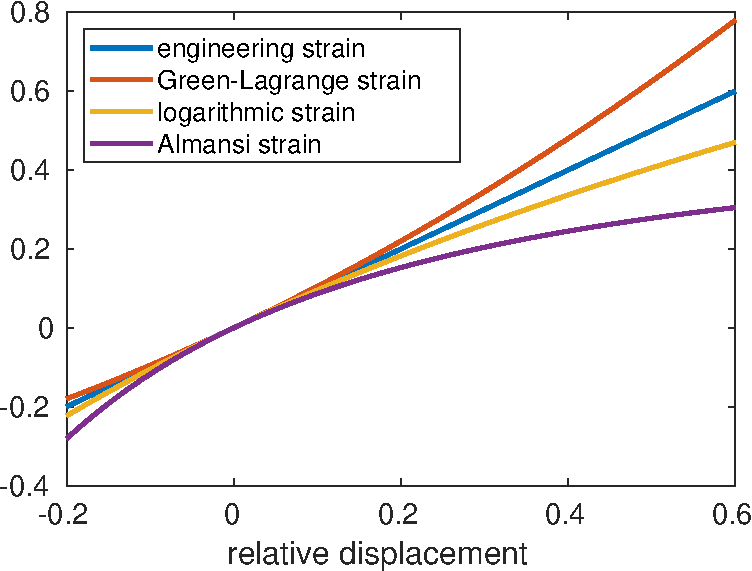
\includegraphics[width=\textwidth]{pic/strainComparison.pdf}
        \end{onlyenv}
      \end{overlayarea}

      \end{column}
    \end{columns}
\end{frame}




\begin{frame}[fragile]
  \frametitle{Slip Systems}
    \begin{columns}
      \begin{column}{0.5\textwidth}
          \begin{overlayarea}{\textwidth}{7.5cm}
            A slip system is specified by a normal direction $\mathbf n$ and a
            slip direction $\mathbf d$ orthogonal to $\mathbf n$
            \vspace{-0.2cm}
  \begin{lstlisting}[style=input]
n = Miller(0,0,0,1,cs,'hkl')
d = Miller(1,1,-2,0,cs,'uvw')
sS = slipSystem(d,n)
\end{lstlisting}

\vspace{0.1cm}

  \begin{onlyenv}<2-> build in fcc, bcc and hcp slip systems \vspace{-0.2cm}
\begin{lstlisting}[style=input]
sS  = slipSystem.pyramidalA(cs)
\end{lstlisting}
  \end{onlyenv}

\vspace{0.1cm}

  \begin{onlyenv}<3>
    symmetrically equivalent slip systems
    \vspace{-0.2cm}
        \begin{lstlisting}[style=input]
sS.symmetrise
        \end{lstlisting}
  \end{onlyenv}
  \begin{onlyenv}<4->
    symmetrically equivalent slip systems
    \vspace{-0.2cm}
        \begin{lstlisting}[style=input]
sS.symmetrise('antipodal')
        \end{lstlisting}
  \end{onlyenv}

\vspace{0.1cm}

  \begin{onlyenv}<5->
    transform to specimen reference frame
    \vspace{-0.2cm}
        \begin{lstlisting}[style=input]
orientation.rand(cs) * sS
        \end{lstlisting}
  \end{onlyenv}

\vspace{0.1cm}

  \begin{onlyenv}<6->
    Schmid or deformation tensor
    \vspace{-0.2cm}
        \begin{lstlisting}[style=input]
m = SchmidTensor(sS)
        \end{lstlisting}
  \end{onlyenv}
  \end{overlayarea}
\end{column}
\begin{column}{0.47\textwidth}
  \vspace{-1.2cm}
  \begin{overlayarea}{\textwidth}{7.5cm}
    \begin{onlyenv}<1-6|handout:0>
      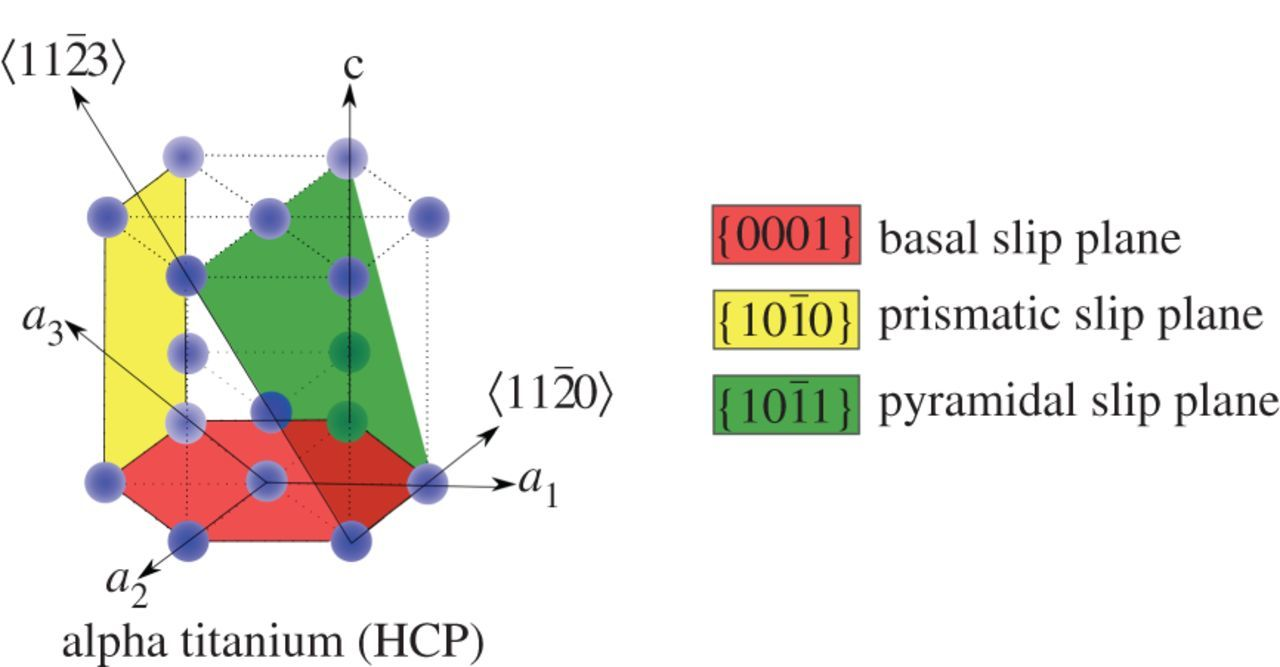
\includegraphics[width=\textwidth]{pic/slip}
      \vspace{-0.5cm}
  \end{onlyenv}
  \begin{onlyenv}<1|handout:0>
\begin{lstlisting}[style=output]
sS = /+slipSystem+/ (/+hcp+/)
 
  U  V  T  W  | H  K  I  L CRSS
  1  1 -2  0    0  0  0  1    1
  \end{lstlisting}
  \end{onlyenv}%
  \begin{onlyenv}<2|handout:0>
\begin{lstlisting}[style=output]
sS = /+slipSystem+/ (/+hcp+/)

  U  V  T  W  | H  K  I  L CRSS
  2 -1 -1  0    0  1 -1  1    1
\end{lstlisting}
  \end{onlyenv}
  \begin{onlyenv}<3>
    \begin{lstlisting}[style=output]
sS = /+slipSystem+/ (/+hcp+/)
 size: 12 x 1 
   U  V  T  W  | H  K  I  L CRSS
  -2  1  1  0    0  1 -1 -1    1
   2 -1 -1  0    0  1 -1 -1    1
  -2  1  1  0    0  1 -1  1    1
   2 -1 -1  0    0  1 -1  1    1
  -1 -1  2  0    1 -1  0  1    1
   1  1 -2  0    1 -1  0  1    1
  -1 -1  2  0   -1  1  0  1    1
   1  1 -2  0   -1  1  0  1    1
  -1  2 -1  0   -1  0  1  1    1
   1 -2  1  0   -1  0  1  1    1
  -1  2 -1  0    1  0 -1  1    1
   1 -2  1  0    1  0 -1  1    1
\end{lstlisting}
  \end{onlyenv}
    \begin{onlyenv}<4|handout:0>
      \begin{lstlisting}[style=output]
sS = /+slipSystem+/ (/+hcp+/)
 size: 6 x 1
 
   U  V  T  W  | H  K  I  L CRSS
  -2  1  1  0    0  1 -1 -1    1
  -2  1  1  0    0  1 -1  1    1
   1  1 -2  0    1 -1  0  1    1
   1  1 -2  0   -1  1  0  1    1
  -1  2 -1  0   -1  0  1  1    1
  -1  2 -1  0    1  0 -1  1    1
\end{lstlisting}
    \end{onlyenv}
    \begin{onlyenv}<5|handout:0>
\begin{lstlisting}[style=output]
ans = /+slipSystem+/ (xyz)

     x     y     z  |    x     y      z
 -0.03 -1.03 -0.97   -1.38  0.74  -0.74
\end{lstlisting}
    \end{onlyenv}
    \begin{onlyenv}<6|handout:0>
\begin{lstlisting}[style=output]
ans = /+velocityGradientTensor+/ (/+hcp+/)
  rank   : 2 (3 x 3)                    
 
 *10^-2
  32.73  56.69  56.69
  -18.9 -32.73 -32.73
      0      0      0
    \end{lstlisting}
    \end{onlyenv}

  \end{overlayarea}
\end{column}
\end{columns}

\end{frame}


\begin{frame}[fragile]
  \frametitle{Schmid Factor}

  \begin{columns}
    \begin{column}{0.5\textwidth}
      \begin{overlayarea}{\textwidth}{7.5cm}
        The Schmid factor is the resolved shear stress $\tau$ for a specific
        tension direction $\mathbf r$
        \begin{equation*}
          \tau = \cos \angle(\mathbf r,\mathbf n) \cdot \cos \angle(\mathbf r,\mathbf d)
          = (\mathbf r^T  \mathbf n) \cdot (\mathbf r^{T}  \mathbf d)
        \end{equation*}
         \vspace{-0.7cm}
\begin{lstlisting}[style=input]
r = vector3d.Z
tau = dot(n,r) .* dot(d,r)
\end{lstlisting}
%
      \begin{onlyenv}<2->
\begin{lstlisting}[style=input]
tau = sS.SchmidFactor(r)
plot(sS.SchmidFactor)
\end{lstlisting}
      \end{onlyenv}

          \vspace{0.2cm}

      \begin{onlyenv}<3|handout:0>
        For general stress $\sigma$ we have $\tau = m : \sigma$
      \vspace{-0.1cm}
\begin{lstlisting}[style=input]
sigma = stressTensor.uniaxial(r)
tau = EinsteinSum(m,[-1 -2],...
              sigma,[-1,-2])
tau = m : sigma
tau = sS.SchmidFactor(sigma)
\end{lstlisting}
    \end{onlyenv}
      \begin{onlyenv}<4->
        For general stress $\sigma$ we have $\tau = m : \sigma$
      \vspace{-0.1cm}
\begin{lstlisting}[style=input]
sigma = stressTensor.uniaxial(r)
tau = (ori * m) : sigma
tau = m : inv(ori) * sigma
\end{lstlisting}
      \begin{onlyenv}<5>
        \begin{lstlisting}[style=input]
tau = SchmidFactor(ori*sS,sigma)
\end{lstlisting}
      \end{onlyenv}

            \end{onlyenv}
    \end{overlayarea}
    \end{column}
    \begin{column}{0.47\textwidth}
      \only<2->{\centering 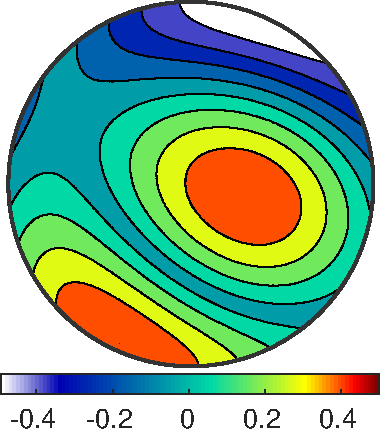
\includegraphics[width=0.8\textwidth]{pic/sFsingle}}
    \end{column}
  \end{columns}
\end{frame}


\begin{frame}[fragile]
  \frametitle{Maximum Schmid Factor}

  \begin{columns}
    \begin{column}{0.7\textwidth}
      \begin{overlayarea}{\textwidth}{7.5cm}
        the Schmid factor for a list of tension directions results in a
        \texttt{length(r)} $\times$ \texttt{length(sS)} matrix \texttt{tau}
        \vspace{-0.2cm}
\begin{lstlisting}[style=input]
sS = sS.symmetrise('antipodal')
r = plotS2Grid('upper')
tau = sS.SchmidFactor(r)
  \end{lstlisting}

\pause
\vspace{0.1cm}
maximum Schmidfactor over the second dimension
\vspace{-0.2cm}
  \begin{lstlisting}[style=input]
[tau_max,id] = max(abs(tau),[],2)
contourf(r,tau_max)
  \end{lstlisting}

\pause

\vspace{0.1cm}
the active slip system
\vspace{-0.2cm}
\begin{lstlisting}[style=input]
contourf(r,id,'contours',12)
hold on
quiver(r,sS(id).n,'color','r');
quiver(r,sS(id).b,'color','g');
hold off

\end{lstlisting}
\end{overlayarea}
\end{column}
\begin{column}{3.8cm}

  \begin{overlayarea}{\textwidth}{8cm}
    \only<2->{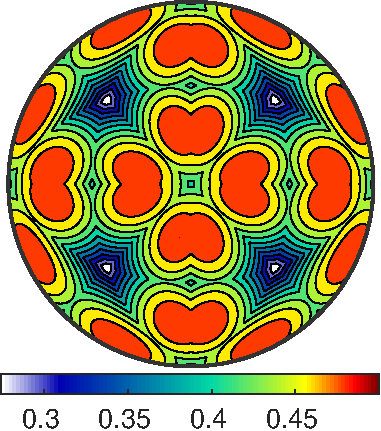
\includegraphics[width=\textwidth]{pic/sFsym}}

    \only<3->{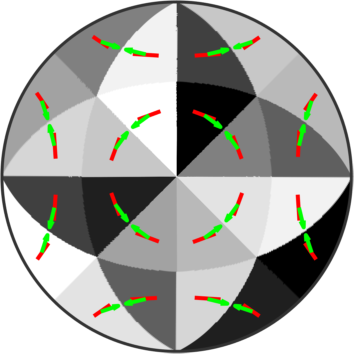
\includegraphics[height=3.5cm]{pic/SFActive.png}}
  \end{overlayarea}

\end{column}
\end{columns}

\end{frame}

  \begin{frame}[fragile]
  \frametitle{Stress Based Analysis - Route 1}
  \vspace{-0.7cm}
  \begin{overlayarea}{\textwidth}{5.1cm}
    \begin{onlyenv}<1->
      \begin{lstlisting}[style=input]
sigma = stressTensor.uniaxial(vector3d.X)
sS = symmetrise(slipSystem.fcc(ebsd.CS))
\end{lstlisting}
  \end{onlyenv}
  \begin{onlyenv}<1|handout:0>
    \vspace{-0.3cm}
    \begin{lstlisting}[style=output]
sS = /+slipSystem+/ (/+fcc+/)
 size: 24 x 1
   u   v   w | h   k   l
   0   1  -1   1   1   1
  -1   0   1   1   1   1
   1  -1   0   1   1   1
   0  -1   1   1   1   1
   1   0  -1   1   1   1
  -1   1   0   1   1   1
   1  -1   0   1   1  -1
   1   0   1   1   1  -1
   0   1   1   1   1  -1
  -1   0  -1   1   1  -1
   0  -1  -1   1   1  -1
  -1   1   0   1   1  -1
   0   1  -1  -1   1   1
   1   0   1  -1   1   1
   1   1   0  -1   1   1
  -1   0  -1  -1   1   1
  -1  -1   0  -1   1   1
   0  -1   1  -1   1   1
  -1   0   1   1  -1   1
   1   1   0   1  -1   1
   0   1   1   1  -1   1
  -1  -1   0   1  -1   1
   0  -1  -1   1  -1   1
   1   0  -1   1  -1   1
\end{lstlisting}
    \end{onlyenv}
    \vspace{-0.35cm}
    \begin{onlyenv}<2->
      \begin{lstlisting}[style=input]
sSGrain = grains.meanOrientation .* sS
\end{lstlisting}
    \end{onlyenv}
    \begin{onlyenv}<2|handout:0>
      \vspace{-0.35cm}
      \begin{lstlisting}[style=output]
sSGrain = /+slipSystem+/ (xyz)
 size: 71 x 24
\end{lstlisting}
    \end{onlyenv}
    \begin{onlyenv}<3->
      \vspace{-0.35cm}
      \begin{lstlisting}[style=input]
SF = sSGrain.SchmidFactor(sigma);
\end{lstlisting}
    \end{onlyenv}
    \begin{onlyenv}<4->
      \vspace{-0.35cm}
      \begin{lstlisting}[style=input]
[maxSF,active] = max(SF,[],2);
plot(grains,maxSF)
\end{lstlisting}
    \end{onlyenv}
    \begin{onlyenv}<5->
      \vspace{-0.35cm}
% \begin{lstlisting}[style=input]
% for id = unique(active)
%   plot(grains(active==id),'FaceColor',color{id},...
%   'DisplayName',[char(nSym(id)) ' ' char(bSym(id))])
% end
% \end{lstlisting}
      \begin{lstlisting}[style=input]
sSactive = grains.meanOrientation .* sS(active);
quiver(grains,sSactive.trace,'color','blue')
quiver(grains,sSactive.b,'color','red')
\end{lstlisting}
\end{onlyenv}
 \end{overlayarea}
 \begin{overlayarea}{\textwidth}{3.5cm}
   \begin{onlyenv}<2-3|handout:0> \centerline{
       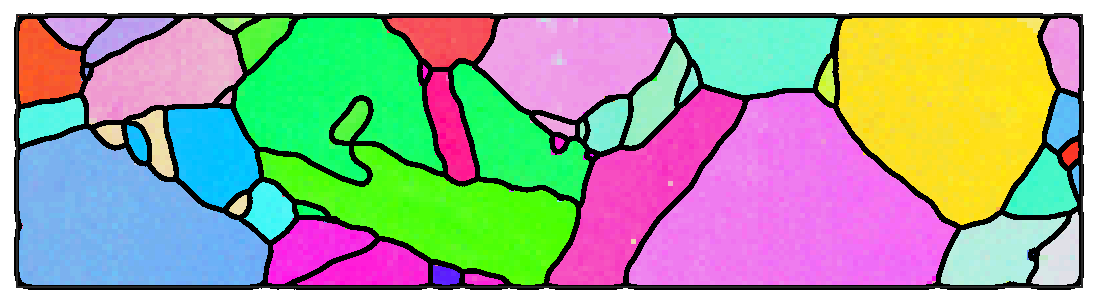
\includegraphics[width=0.9\textwidth]{pic/ebsdCSL.pdf}}
   \end{onlyenv}
   \begin{onlyenv}<4|handout:0> \centerline{
       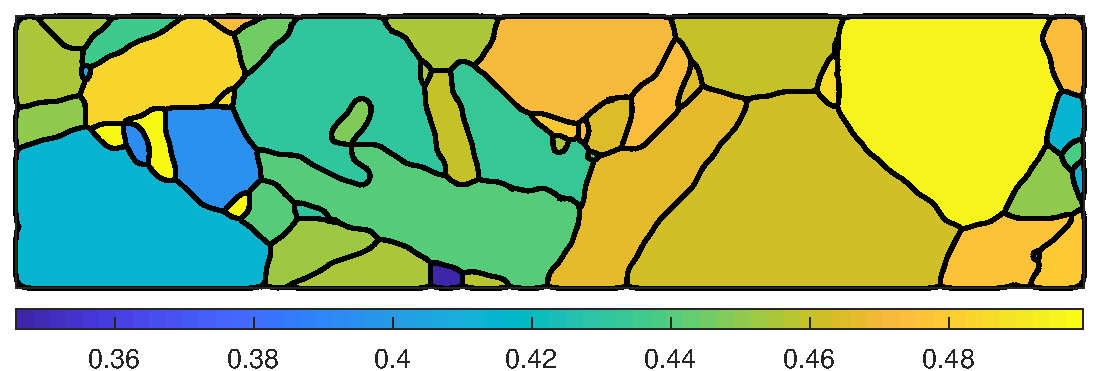
\includegraphics[width=0.9\textwidth]{pic/ebsdSF.pdf}}
   \end{onlyenv}
   \begin{onlyenv}<5> \centerline{
       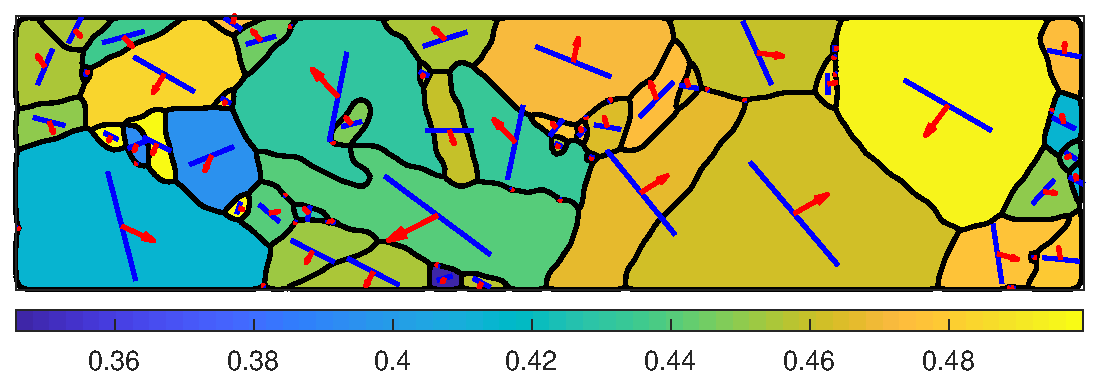
\includegraphics[width=0.9\textwidth]{pic/ebsdSS.pdf}}
   \end{onlyenv}
 \end{overlayarea}

\end{frame}



\begin{frame}[fragile]
  \frametitle{Stress Based Analysis - Route 2}
  \vspace{-0.5cm}
  \begin{overlayarea}{\textwidth}{4.8cm}
    \begin{onlyenv}<1->
\begin{lstlisting}[style=input]
sigma = stressTensor.uniaxial(vector3d.X)
\end{lstlisting}
  \end{onlyenv}
  \begin{onlyenv}<1|handout:0>
    \vspace{-0.35cm}
\begin{lstlisting}[style=output]
sigma = /+stressTensor+/ (xyz)
  rank: 2 (3 x 3)

 1 0 0
 0 0 0
 0 0 0
\end{lstlisting}
    \end{onlyenv}
    \vspace{-0.35cm}
    \begin{onlyenv}<2->
\begin{lstlisting}[style=input]
sigmaCrystal = inv(grains.meanOrientation) * sigma
\end{lstlisting}
    \end{onlyenv}
    \begin{onlyenv}<2|handout:0>
      \vspace{-0.35cm}
\begin{lstlisting}[style=output]
sigmaCrystal = /+stressTensor+/ (/+iron+/)
  size   : 71 x 1
  rank   : 2 (3 x 3)
\end{lstlisting}
    \end{onlyenv}
    \begin{onlyenv}<3->
      \vspace{-0.35cm}
      \begin{lstlisting}[style=input]
SF = sS.SchmidFactor(sigmaCrystal);
\end{lstlisting}
    \end{onlyenv}
    \begin{onlyenv}<4->
      \vspace{-0.35cm}
      \begin{lstlisting}[style=input]
[maxSF,active] = max(abs(SF),[],2);
plot(grains,maxSF)
\end{lstlisting}
    \end{onlyenv}
    \begin{onlyenv}<5->
      \vspace{-0.35cm}
% \begin{lstlisting}[style=input]
% for id = unique(active)
%   plot(grains(active==id),'FaceColor',color{id},...
%   'DisplayName',[char(nSym(id)) ' ' char(bSym(id))])
% end
% \end{lstlisting}
      \begin{lstlisting}[style=input]
sSactive = grains.meanOrientation .* sS(active);
quiver(grains,sSactive.trace,'color','blue')
quiver(grains,sSactive.b,'color','red')
\end{lstlisting}
\end{onlyenv}
\end{overlayarea}

\begin{overlayarea}{\textwidth}{3.5cm}
  \begin{onlyenv}<1-3|handout:0> \centerline{
      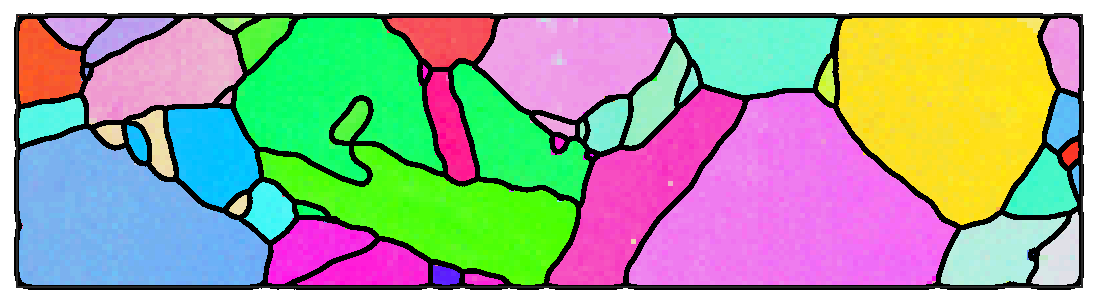
\includegraphics[width=0.9\textwidth]{pic/ebsdCSL.pdf}}
  \end{onlyenv}
  \begin{onlyenv}<4|handout:0> \centerline{
      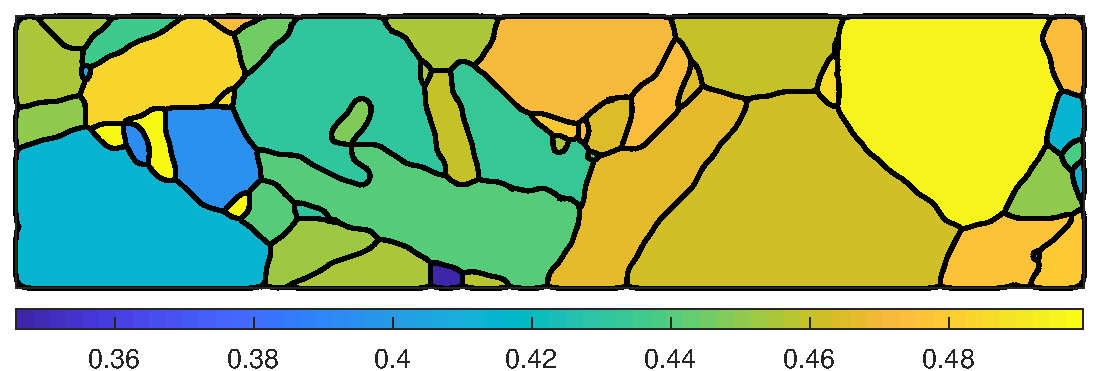
\includegraphics[width=0.9\textwidth]{pic/ebsdSF.pdf}}
  \end{onlyenv}
  \begin{onlyenv}<5> \centerline{
      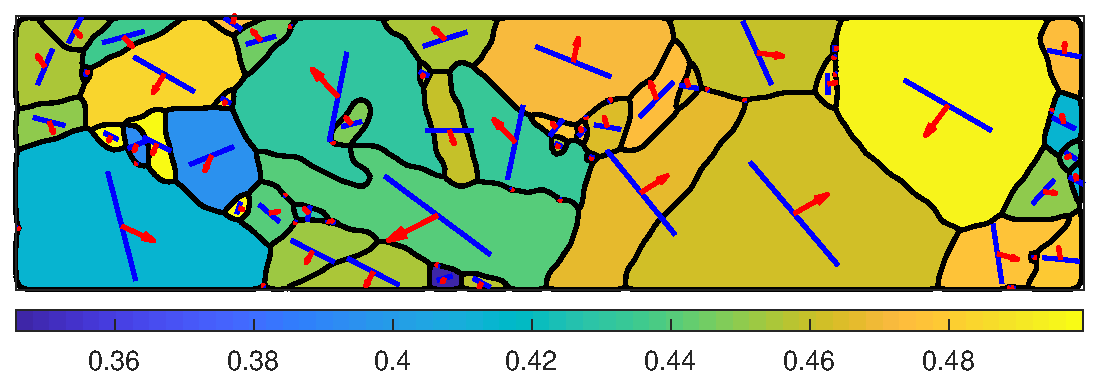
\includegraphics[width=0.9\textwidth]{pic/ebsdSS.pdf}}
  \end{onlyenv}
\end{overlayarea}

  \end{frame}


% \subsection*{Plastic deformation - stress based analysis}

% \begin{frame}[fragile]
%   \frametitle{Plastic deformation - stress based analysis}

% convert slip systems to specimen coordinates:
% \vspace{-0.2cm}
% \begin{lstlisting}[style=input]
% ori = grains.meanOrientation;
% sSGrains =  ori * sS
% \end{lstlisting}
%       \begin{onlyenv}<1>
%         \vspace{-0.2cm}
%       \begin{lstlisting}[style=output]
% sSGrains = /+slipSystem+/ (show methods, plot)
%  size: 37 x 12
%       \end{lstlisting}
%     \end{onlyenv}

% \pause
% \begin{columns}
%   \begin{column}{0.65\textwidth}

% some uniaxial stress:
% \vspace{-0.2cm}
%   \begin{lstlisting}[style=input]
% sigma = tensor.diag([1,0,0])
% \end{lstlisting}
%       \begin{onlyenv}<2>
%         \vspace{-0.2cm}
%         \begin{lstlisting}[style=output]
% sigma = /+tensor+/ (show methods, plot)
%   rank: 2 (3 x 3)

%  1 0 0
%  0 0 0
%  0 0 0
%       \end{lstlisting}
%     \end{onlyenv}

% \pause

% the Schmid Factor for each slip system:
% \vspace{-0.2cm}
% \begin{lstlisting}[style=input]
% SF = sSGrains.SchmidFactor(sigma)
% \end{lstlisting}

% \pause

% determine for each grain the active slip system
% \vspace{-0.2cm}
% \begin{lstlisting}[style=input]
% [maxSF,active] = max(SF,[],2);
% plot(grains,maxSF)
% \end{lstlisting}

% \pause

% plot slip direction and slip plane
% \vspace{-0.2cm}
% \begin{lstlisting}[style=input]
% sSActive = ori .* sS(active)
% quiver(grains,sSActive.b)
% quiver(grains,sSActive.n)
% \end{lstlisting}

% \end{column}
% \begin{column}{0.35\textwidth}
%   \only<4>{\includegraphics[width=\textwidth]{pic/SF.png}}
%   \only<5>{\includegraphics[width=\textwidth]{pic/SFSlip.png}}
% \end{column}
% \end{columns}

% \end{frame}


\begin{frame}[fragile]
  \frametitle{Strain Based Analysis}
  \vspace{-0.5cm}
  \begin{overlayarea}{\textwidth}{4.8cm}
    \begin{onlyenv}<1->
\begin{lstlisting}[style=input]
eps = strainTensor(diag([1,0,-1])
\end{lstlisting}
  \end{onlyenv}
  \begin{onlyenv}<1|handout:0>
    \vspace{-0.35cm}
\begin{lstlisting}[style=output]
sigma = /+strainTensor+/ (xyz)
  rank: 2 (3 x 3)

 1  0  0
 0  0  0
 0  0 -1
\end{lstlisting}
    \end{onlyenv}
    \vspace{-0.35cm}
    \begin{onlyenv}<2->
\begin{lstlisting}[style=input]
epsCrystal = inv(grains.meanOrientation) * eps
\end{lstlisting}
    \end{onlyenv}
    \begin{onlyenv}<2|handout:0>
      \vspace{-0.35cm}
\begin{lstlisting}[style=output]
epsCrystal = /+strainTensor+/ (/+iron+/)
  size   : 71 x 1
  rank   : 2 (3 x 3)
\end{lstlisting}
    \end{onlyenv}
    \begin{onlyenv}<3->
      \vspace{-0.35cm}
      \begin{lstlisting}[style=input]
[TF, b, W] = calcTaylor(epsCrystal, sS);
      \end{lstlisting}
    \end{onlyenv}
    \begin{onlyenv}<4->
      \vspace{-0.35cm}
      \begin{lstlisting}[style=input]
plot(grains,TF)
\end{lstlisting}
    \end{onlyenv}
    \begin{onlyenv}<5->
      \vspace{-0.35cm}
      \begin{lstlisting}[style=input]
[bMax ,bMaxId] = max(b,[],2);
sSactive = grains.meanOrientation .* sS(bMaxId);
quiver(grains,sSactive.b,'color','red')
quiver(grains,sSactive.trace,'color','blue')
\end{lstlisting}
\end{onlyenv}
\end{overlayarea}

\begin{overlayarea}{\textwidth}{3.5cm}
  \begin{onlyenv}<1-3|handout:0> \centerline{
      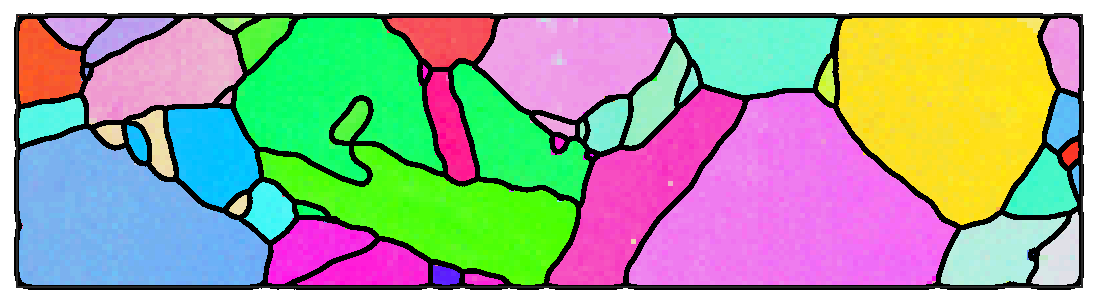
\includegraphics[width=0.9\textwidth]{pic/ebsdCSL.pdf}}
  \end{onlyenv}
  \begin{onlyenv}<4|handout:0> \centerline{
      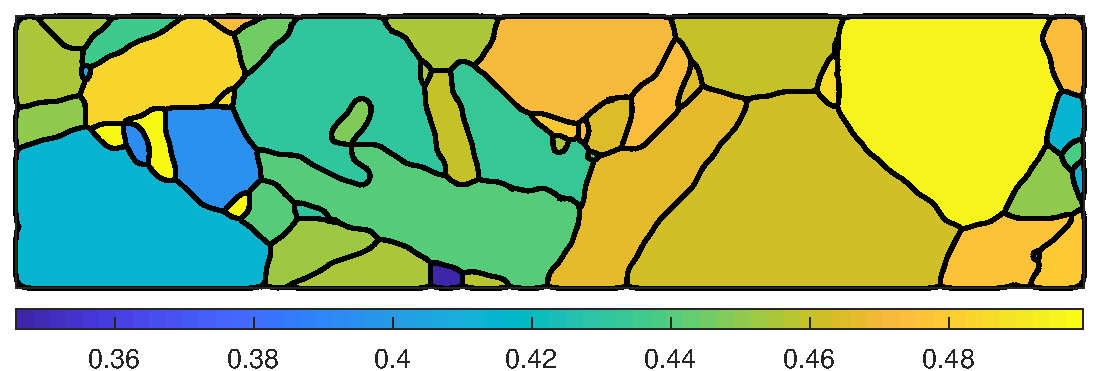
\includegraphics[width=0.9\textwidth]{pic/ebsdSF.pdf}}
  \end{onlyenv}
  \begin{onlyenv}<5> \centerline{
      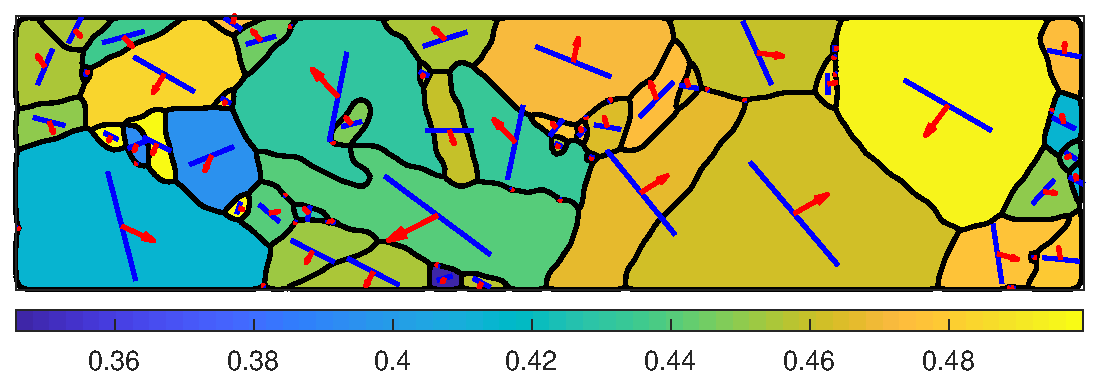
\includegraphics[width=0.9\textwidth]{pic/ebsdSS.pdf}}
  \end{onlyenv}
\end{overlayarea}

  \end{frame}



% \begin{frame}[fragile]
%   \frametitle{Plastic deformation - strain based analysis}

% some strain:
% \vspace{-0.2cm}
%       \begin{lstlisting}[style=input]
% q = 0.25; eps = strainTensor.diag([1 -q -(1-q)])
%       \end{lstlisting}
%       \begin{onlyenv}<1>
%         \vspace{-0.2cm}
%         \begin{lstlisting}[style=output]
% eps = /+strainTensor+/ (show methods, plot)
%   rank: 2 (3 x 3)
%   rank: 2 (3 x 3)

%      1     0     0
%      0 -0.25     0
%      0     0 -0.75
%    \end{lstlisting}
%     \end{onlyenv}

% \pause

%     transform strain to crystal coordinates
%     \vspace{-0.2cm}
%       \begin{lstlisting}[style=input]
% ori = grains('fcc').meanOrientation
% epsGrain = inv(ori) * eps
%       \end{lstlisting}
%       \begin{onlyenv}<2>
%         \vspace{-0.2cm}
%         \begin{lstlisting}[style=output]
% epsGrain = /+strainTensor+/ (show methods, plot)
%   size   : 37 x 1
%   rank   : 2 (3 x 3)
%   mineral: Austenite (fcc, 432)
%         \end{lstlisting}
%       \end{onlyenv}

%       \pause

% compute Taylor factor
%       \vspace{-0.2cm}
% \begin{lstlisting}[style=input]
% [M,b,mori] = calcTaylor(epsGrain,sS);
% \end{lstlisting}

%   \begin{columns}
%     \begin{column}{0.62\textwidth}

%         \vspace{-0.5cm}
% \begin{lstlisting}[style=input]
% plot(grains,M)
%       \end{lstlisting}

%       \pause

%       \begin{lstlisting}[style=input]
% [bMax,bMaxId] = max(b,[],2);
% sSGrains = ori .* sS(bMaxId);
% hold on
% quiver(grains,sSGrains.b)
% quiver(grains,sSGrains.n)
% hold off
% \end{lstlisting}


%     \end{column}
%      \begin{column}{0.35\textwidth}
%        \only<3>{\includegraphics[width=\textwidth]{pic/taylor.png}}
%        \only<4>{\includegraphics[width=\textwidth]{pic/taylorSlip.png}}
%      \end{column}
%    \end{columns}
% %   \end{overlayarea}
% \end{frame}

\begin{frame}[fragile]
  \frametitle{Rolling texture evolution}

  \begin{columns}
    \begin{column}{0.73\textwidth}

      \vspace{-0.7cm}
      \begin{overlayarea}{\textwidth}{8cm}

\begin{lstlisting}[style=input]
ori = orientation.rand(10000,CS)
h = Miller({0,0,1},{1,1,1}),CS)
plotPDF(ori,'contourf')
\end{lstlisting}

\pause

the slip systems
\vspace{-0.2cm}
        \begin{lstlisting}[style=input]
sS=symmetrise(slipSystem.fcc(CS))
      \end{lstlisting}

      \begin{onlyenv}<2|handout:0>
        \vspace{-0.2cm}
      \begin{lstlisting}[style=output]
sS = /+slipSystem+/ (/+Austenite (fcc)+/)
 size: 12 x 1
   u   v   w | h   k   l
   0   1  -1   1   1   1
  -1   0   1   1   1   1
   1  -1   0   1   1   1
   1  -1   0   1   1  -1
   1   0   1   1   1  -1
   0   1   1   1   1  -1
   0   1  -1  -1   1   1
   1   0   1  -1   1   1
   1   1   0  -1   1   1
  -1   0   1   1  -1   1
   1   1   0   1  -1   1
   0   1   1   1  -1   1
      \end{lstlisting}
    \end{onlyenv}

    \pause

30 percent strain
\vspace{-0.2cm}
\begin{lstlisting}[style=input]
eps = strainTensor(diag([0.3 0 -0.3])) / 10
\end{lstlisting}

\pause

iterate deformation:
\vspace{-0.2cm}
      \begin{lstlisting}[style=input]
for i = 1:10
  [TF,b,W] = calcTaylor( inv(ori) * eps, sS);
  ori = ori .* orientation(-W);
  plotPDF(ori,h,'contourf')
end
\end{lstlisting}

\only<4|handout:0>{i=1}
\only<5|handout:0>{i=2}
\only<6|handout:0>{i=3}
\only<7|handout:0>{i=4}
\only<8|handout:0>{i=5}
\only<9|handout:0>{i=6}
\only<10|handout:0>{i=7}
\only<11|handout:0>{i=8}
\only<12|handout:0>{i=9}
\only<13|handout:0>{i=10}

\end{overlayarea}
\end{column}
\begin{column}{0.24\textwidth}
  \begin{overlayarea}{\textwidth}{8cm}
    \vspace{-1cm}
    \begin{onlyenv}<1-3|handout:0>
      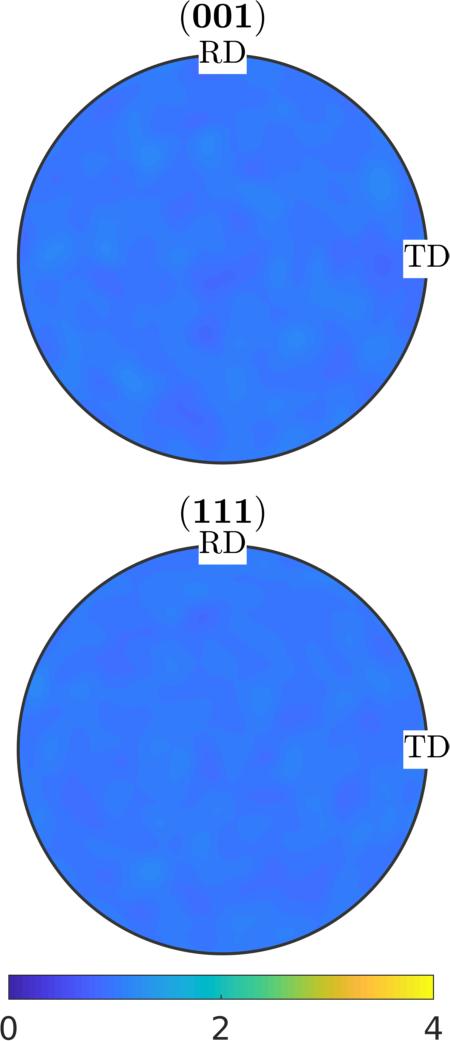
\includegraphics[width=\textwidth]{pic/rolling001_0.png}
    \end{onlyenv}

    \begin{onlyenv}<4|handout:0>
      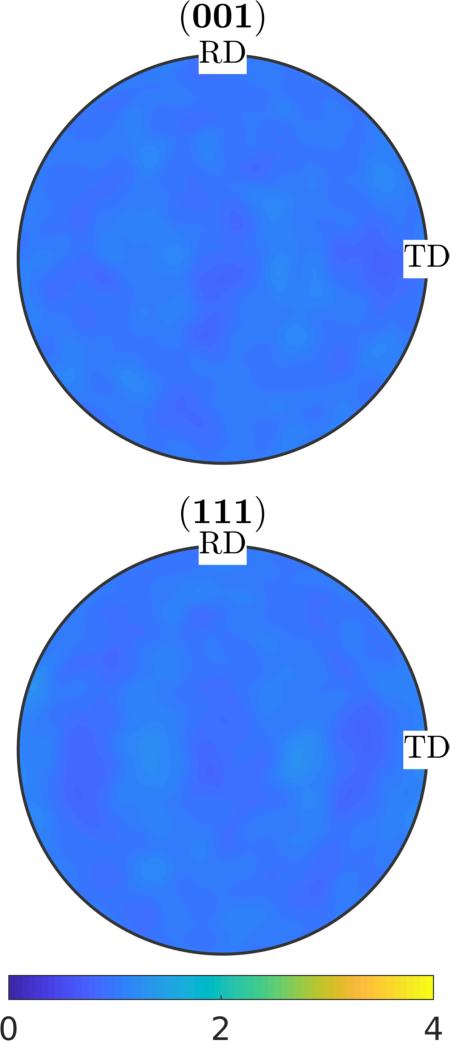
\includegraphics[width=\textwidth]{pic/rolling001_1.png}
    \end{onlyenv}

    \begin{onlyenv}<5|handout:0>
      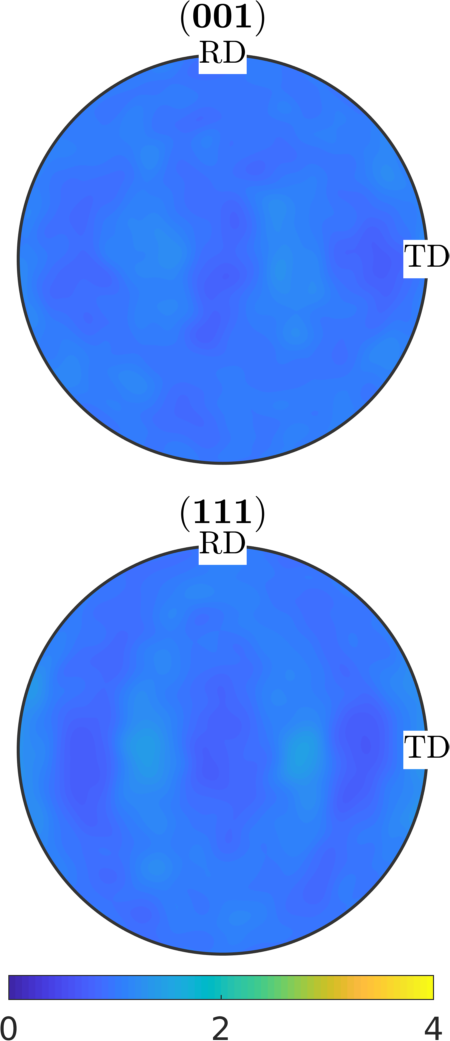
\includegraphics[width=\textwidth]{pic/rolling001_2.png}
    \end{onlyenv}

    \begin{onlyenv}<6|handout:0>
      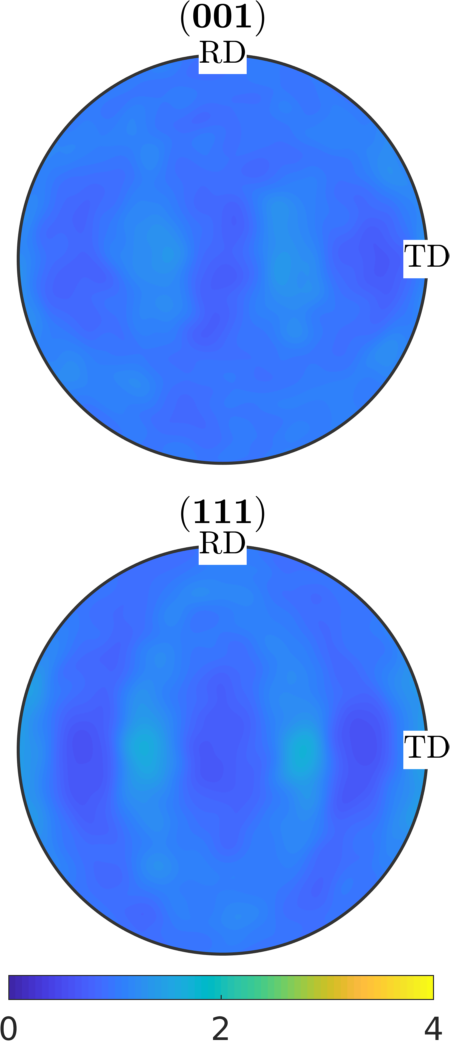
\includegraphics[width=\textwidth]{pic/rolling001_3.png}
    \end{onlyenv}

    \begin{onlyenv}<7|handout:0>
      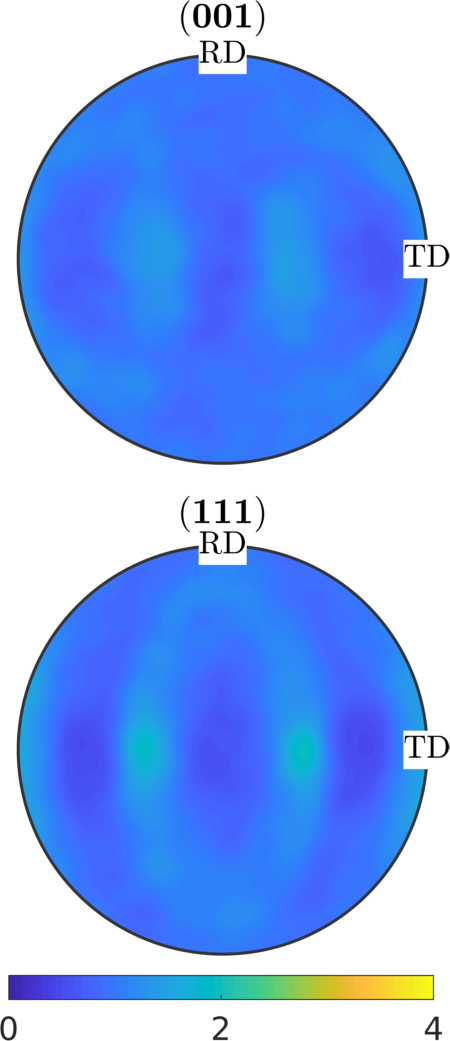
\includegraphics[width=\textwidth]{pic/rolling001_4.png}
    \end{onlyenv}

    \begin{onlyenv}<8|handout:0>
      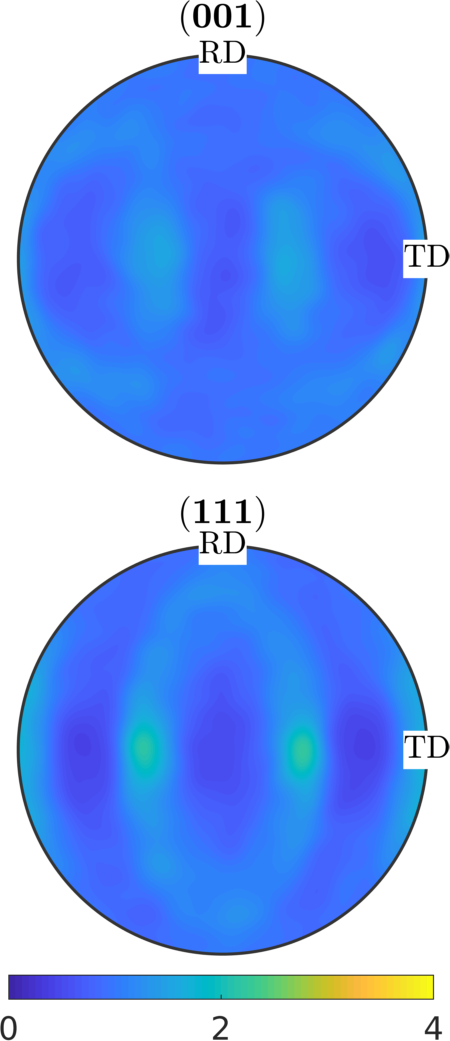
\includegraphics[width=\textwidth]{pic/rolling001_5.png}
    \end{onlyenv}

    \begin{onlyenv}<9|handout:0>
      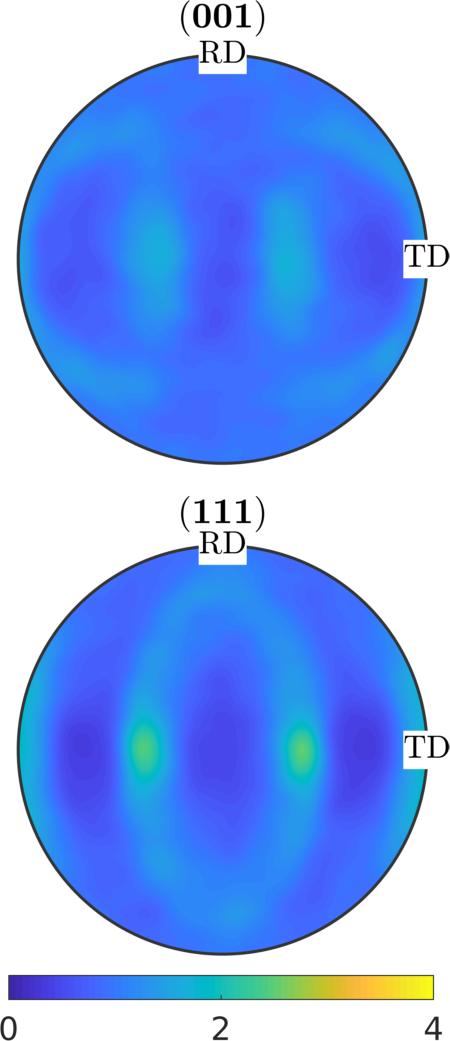
\includegraphics[width=\textwidth]{pic/rolling001_6.png}
    \end{onlyenv}

    \begin{onlyenv}<10|handout:0>
      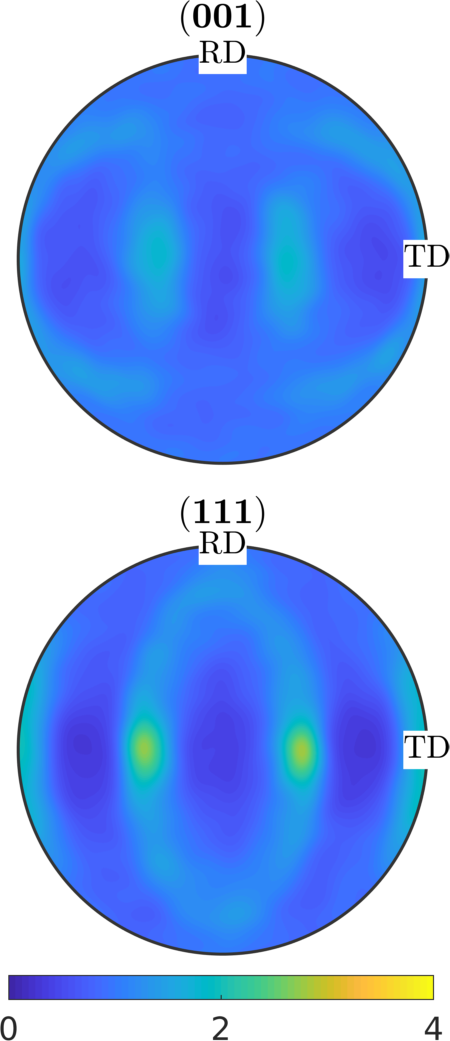
\includegraphics[width=\textwidth]{pic/rolling001_7.png}
    \end{onlyenv}

    \begin{onlyenv}<11|handout:0>
      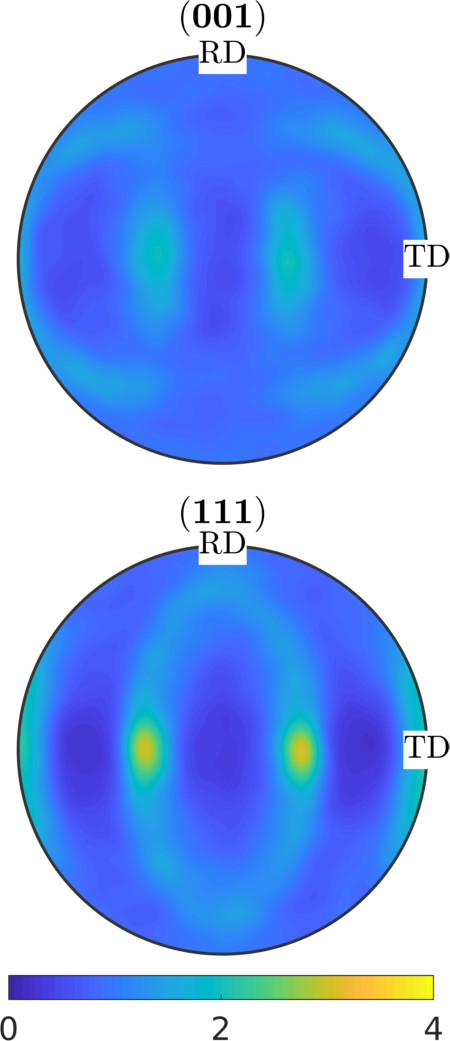
\includegraphics[width=\textwidth]{pic/rolling001_8.png}
    \end{onlyenv}

    \begin{onlyenv}<12|handout:0>
      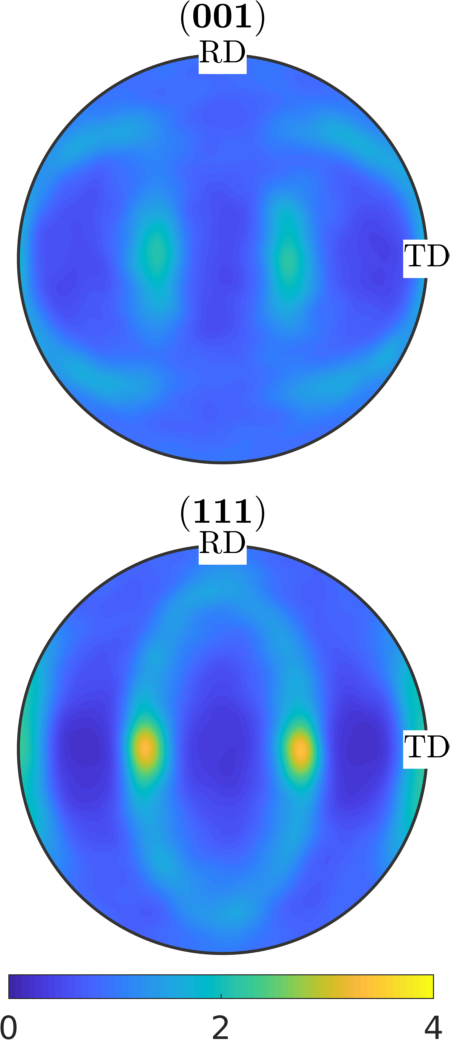
\includegraphics[width=\textwidth]{pic/rolling001_9.png}
    \end{onlyenv}

    \begin{onlyenv}<13>
      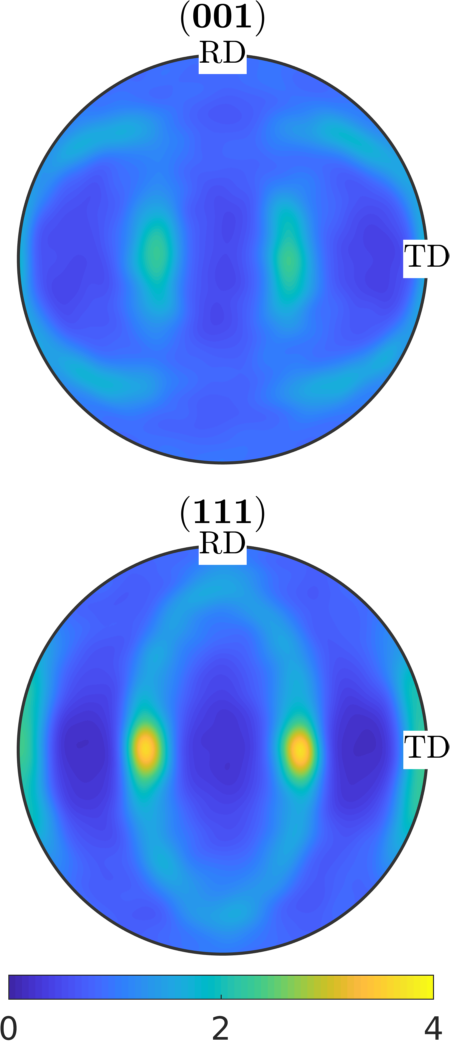
\includegraphics[width=\textwidth]{pic/rolling001_10.png}
    \end{onlyenv}
  \end{overlayarea}
\end{column}
   \end{columns}
%   \end{overlayarea}
\end{frame}


\begin{frame}[fragile]
  \frametitle{Texture Evolution - The Traditional Route}

  \begin{columns}
    \begin{column}{0.41 \textwidth}      
      \begin{overlayarea}{\textwidth}{0.85\textheight}
        \vspace{-0.5cm}
        \structure{Ingredients}
        \begin{itemize}
        \item<1-> family of slip systems $(b_{\ell},n_{\ell})$
        \item<1-> Schmid tensors
          $S_{\ell} = b_{\ell} \otimes d_{\ell}$
        \item<2-> strain tensor $\varepsilon$
        \item<3-> deformation law $\Omega(\mathtt{ori})$
        \item<4-> initial ODF $f_{0}$  
        \end{itemize}

        \medskip

        \structure{Algorithm}
        \begin{itemize}    
        \item[1.]<5-> simulate orientations $\mathtt{ori}_{k}^{0}$
        \item[2.]<6-> update $\mathtt{ori}_{k}^{1} = \mathtt{ori}_{k}^{0} +
          \Omega(\mathtt{ori}_{k}^{0})$
        \item[3.]<7-> estimate ODF $f^{1}$ from $\mathtt{ori}_{k}^{1}$
        \end{itemize}

        \medskip

        \begin{onlyenv}<8>
        \structure{Problems}
        \begin{itemize}
           \item many orientations $\mathtt{ori}_{k}^{0}$ required
           \item slow computation of $\Omega(\mathtt{ori}_{k}^{0})$
           \item ODF estimation not so easy
           \end{itemize}  
        \end{onlyenv}
        
         \end{overlayarea}
       \end{column}
    \begin{column}{0.57 \textwidth}
      \begin{overlayarea}{\textwidth}{0.85\textheight}
        \vspace{-0.5cm}
\begin{lstlisting}[style=input]
cs = crystalSymmetry('222',[5 10 6])
sS = slipSystem({1,0,0},{0,0,1},cs)
S  = sS.SchmidTensor
\end{lstlisting}
        \vspace{-0.3cm}
        \begin{onlyenv}<1>
\begin{lstlisting}[style=output]
S = /+velocityGradientTensor+/ (olivine)
  rank: 2 (3 x 3)
 
 0 0 1
 0 0 0
 0 0 0
\end{lstlisting}
        \end{onlyenv}
         \begin{onlyenv}<2->
\begin{lstlisting}[style=input]
eps = strainTensor(diag(0.3,0,-0.3))
\end{lstlisting}
         \end{onlyenv}
         \begin{onlyenv}<3->
           \begin{equation*}
             \Omega(\mathtt{ori}) = (S_{\mathtt{even}}(\mathtt{ori}):\varepsilon) \cdot S_{\mathtt{odd}}
           \end{equation*}           
         \end{onlyenv}
         \begin{onlyenv}<3>
           \begin{center}
             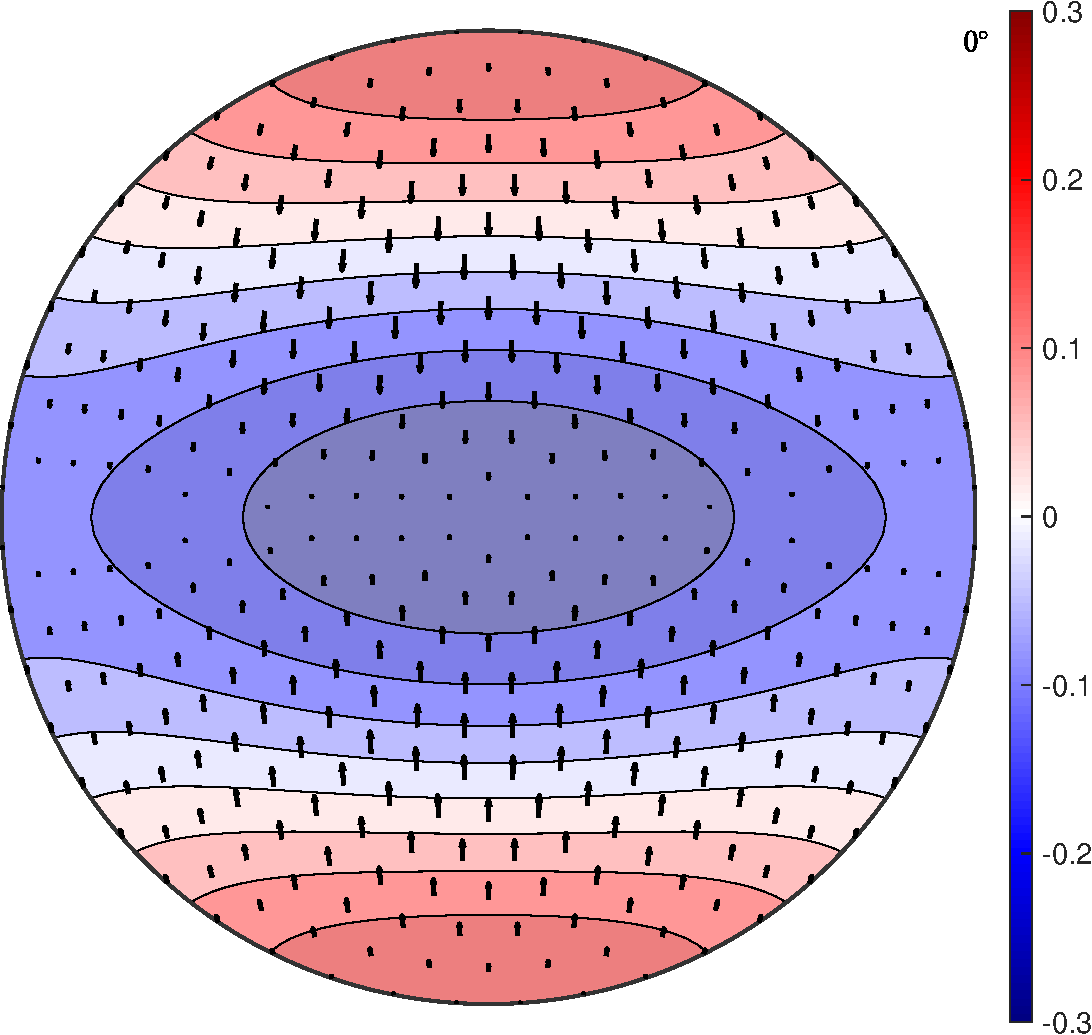
\includegraphics[height=0.5\textheight]{pic/Omega.pdf}
           \end{center}
         \end{onlyenv}%
         \begin{onlyenv}<4>
           \begin{center}
             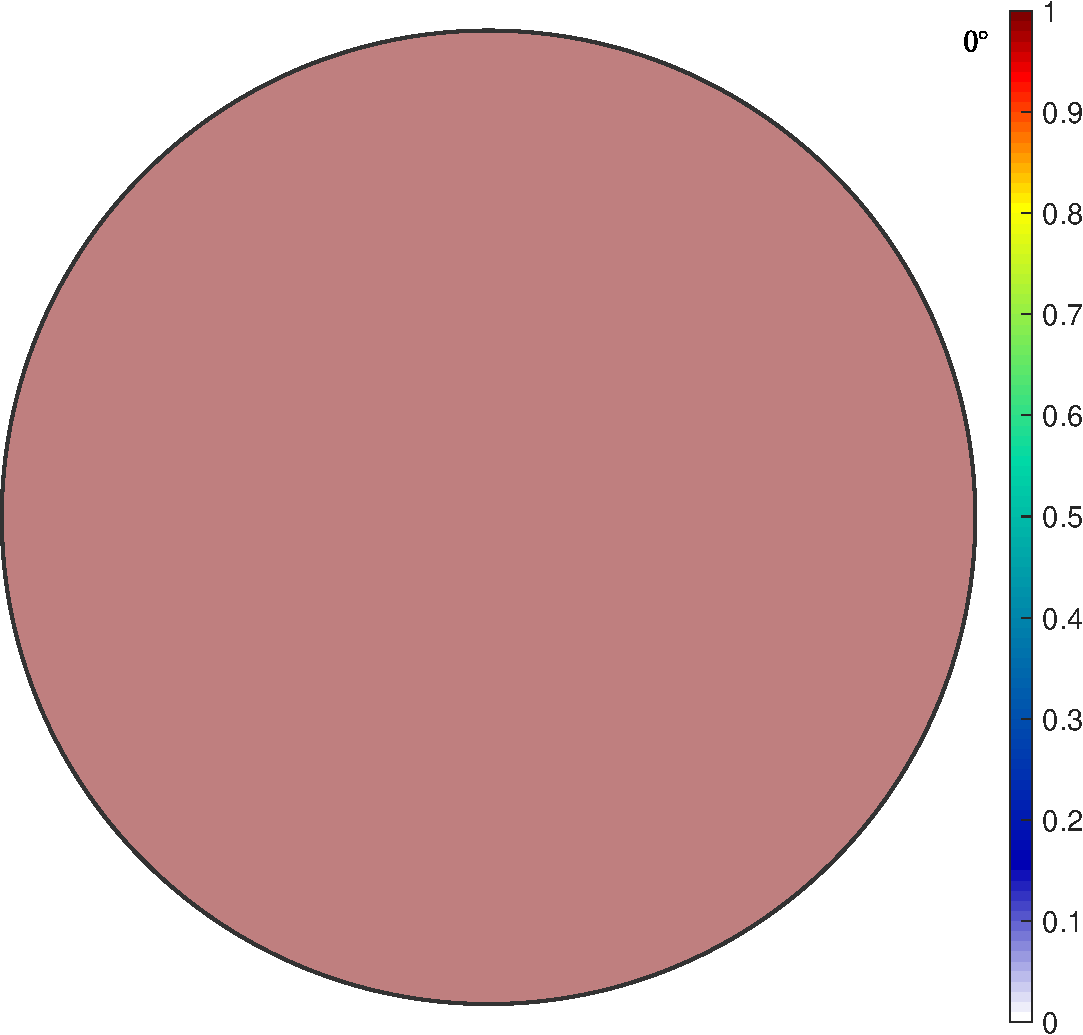
\includegraphics[height=0.5\textheight]{pic/odf0.pdf}
           \end{center}
         \end{onlyenv}%
         \begin{onlyenv}<5>
           \begin{center}
             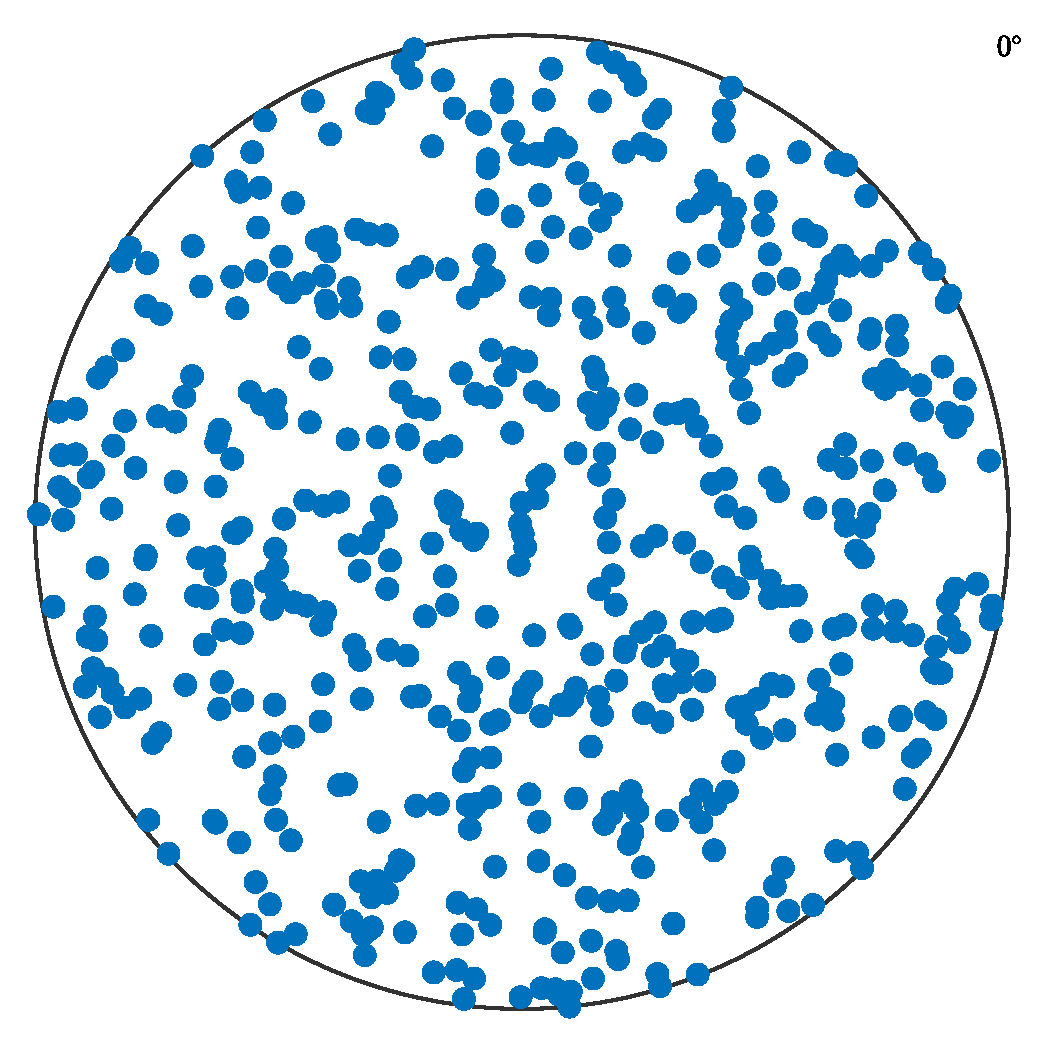
\includegraphics[height=0.5\textheight]{pic/ori0.pdf}
           \end{center}
         \end{onlyenv}%
         \begin{onlyenv}<6>
           \begin{center}
             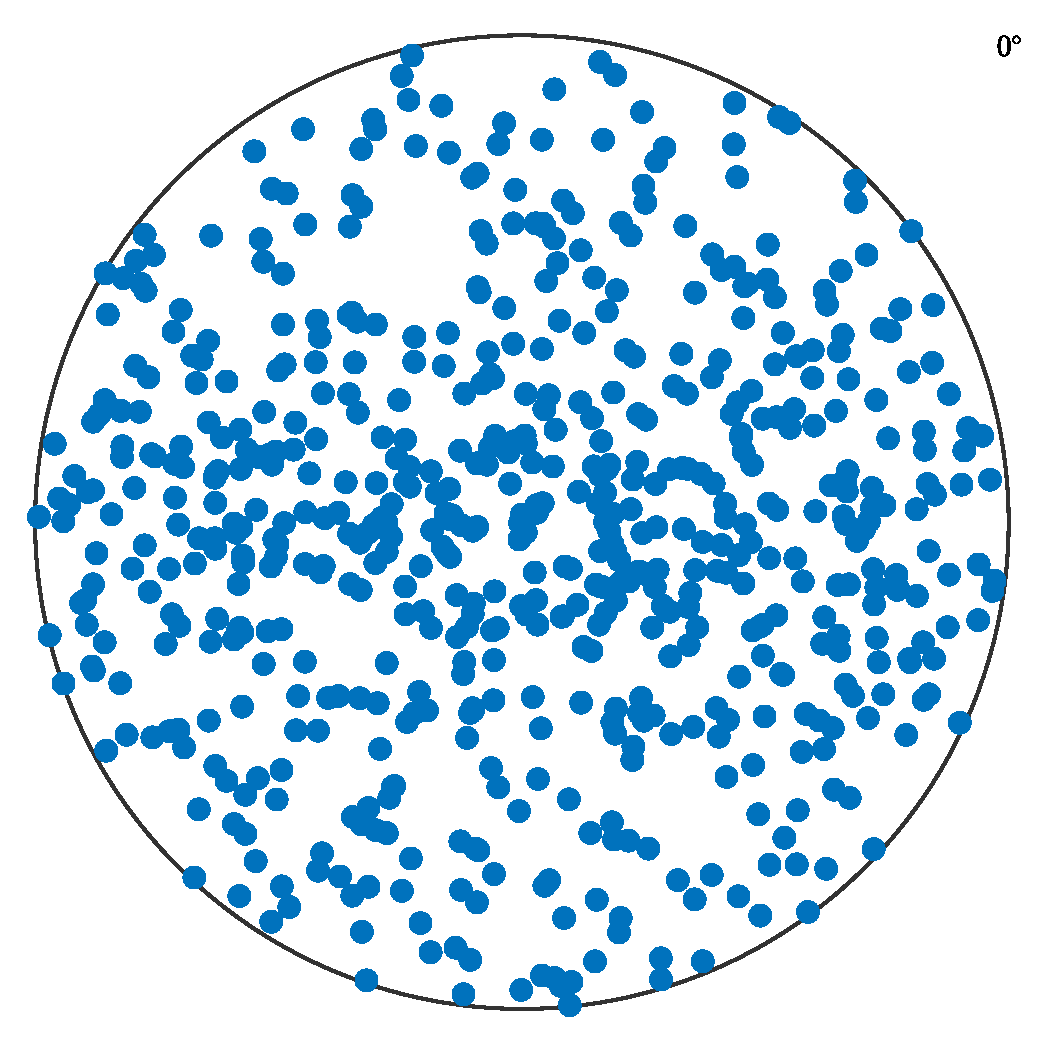
\includegraphics[height=0.5\textheight]{pic/ori1.pdf}
           \end{center}
         \end{onlyenv}%
         \begin{onlyenv}<7>
           \begin{center}
             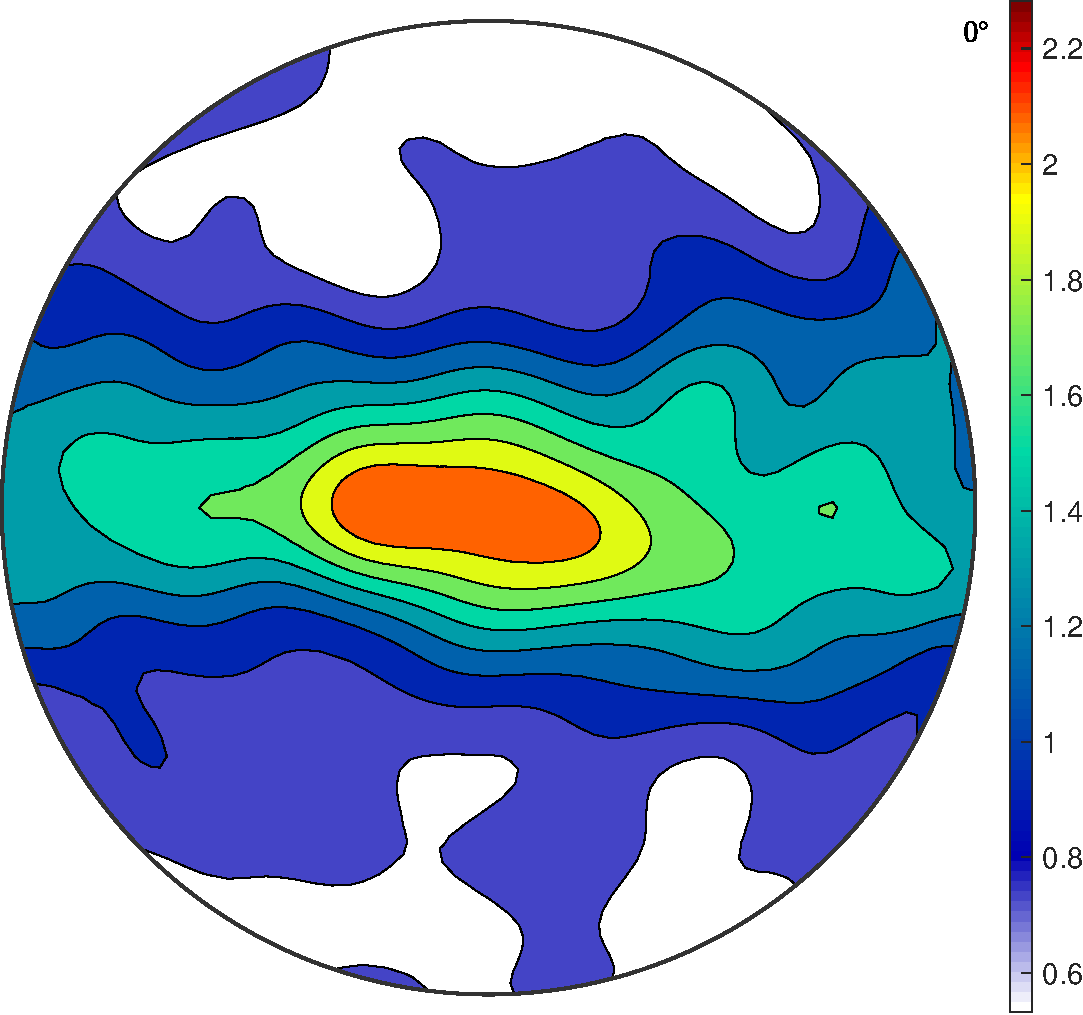
\includegraphics[height=0.5\textheight]{pic/odf1.pdf}
           \end{center}
         \end{onlyenv}%
         \begin{onlyenv}<8>
           \begin{center}
             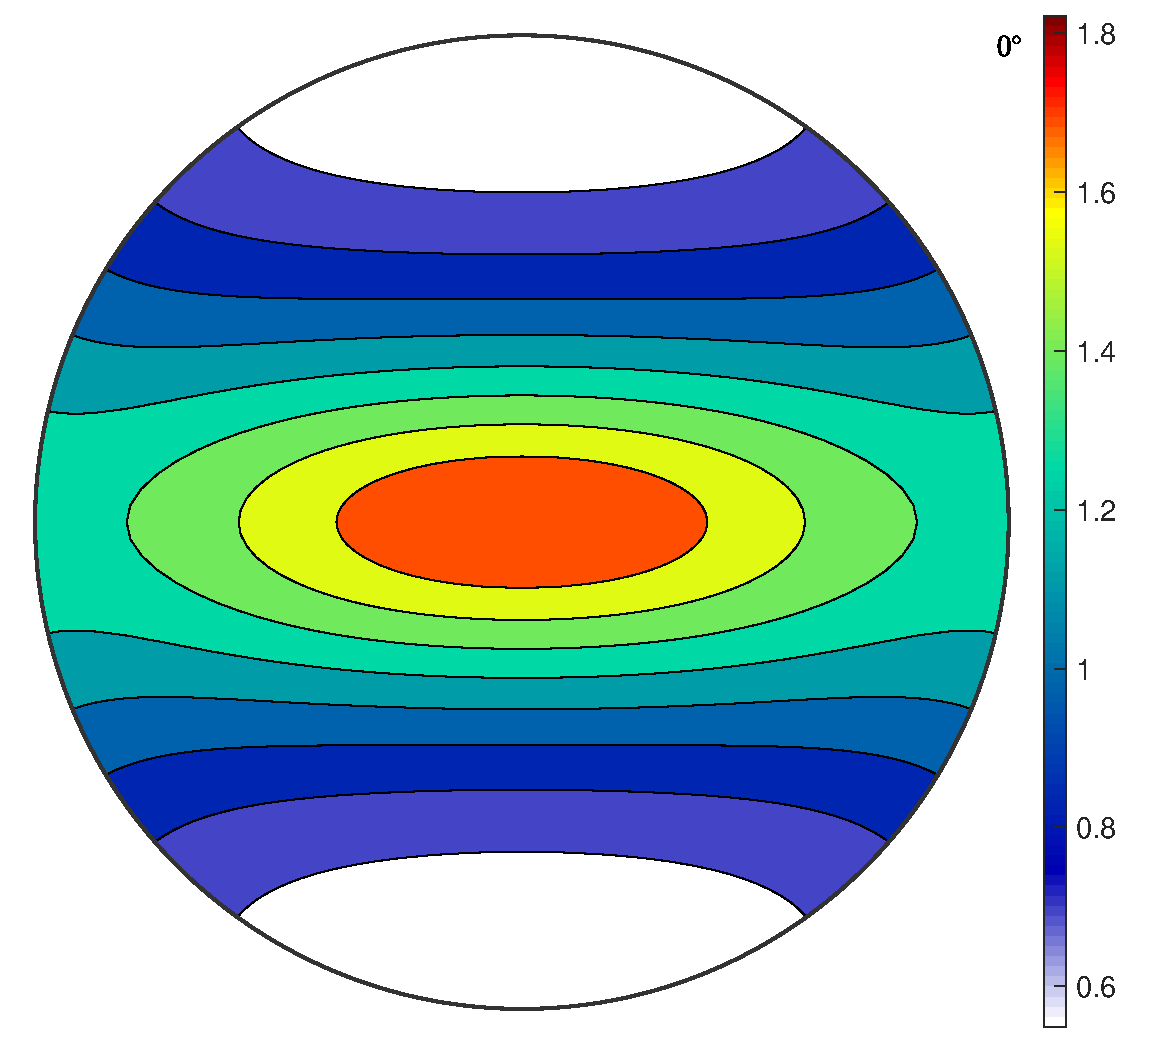
\includegraphics[height=0.5\textheight]{pic/odfTrue.pdf}
           \end{center}
         \end{onlyenv}%
       \end{overlayarea}
    \end{column}
  \end{columns}
\end{frame}


\begin{frame}
  \frametitle{The Transport Equation}
\begin{columns}
    \begin{column}{0.6 \textwidth}      
      \begin{overlayarea}{\textwidth}{0.85\textheight}
        \vspace{-0.5cm}  
  \begin{block}{The continuity or transport equation}
    \begin{equation*}
      \frac{\partial}{\partial t} f = -\text{div} (f \cdot  \Omega)
    \end{equation*}
    describes the change of the ODF $f(\mathtt{ori},t)$ at time $t$ with
    respect to the
    spin tensor $\Omega(\mathtt{ori})$
    
    % \begin{itemize}
    % \item $o$ - orientation
    % \paritem $f(o,t)$ - ODF at time $t$
    % \paritem $\Omega(o)$ - local spin tensor
    % \end{itemize}    
  \end{block}

  \begin{onlyenv}<2->
    \begin{block}{Euler method}
      \begin{itemize}
      \item start with an initial odf $f_{0}$
      \item for $k=1,\ldots,N$ do
        \begin{equation*}
          f_{k} = f_{k-1} - \frac{1}{N} \text{div} (f_{k} \cdot  \Omega) 
        \end{equation*}
      \end{itemize}
    \end{block}
  \end{onlyenv}

\end{overlayarea}  
\end{column}
\begin{column}{0.3\textwidth}
  \begin{overlayarea}{\textwidth}{0.85\textheight}
    \vspace{-1.5cm}

      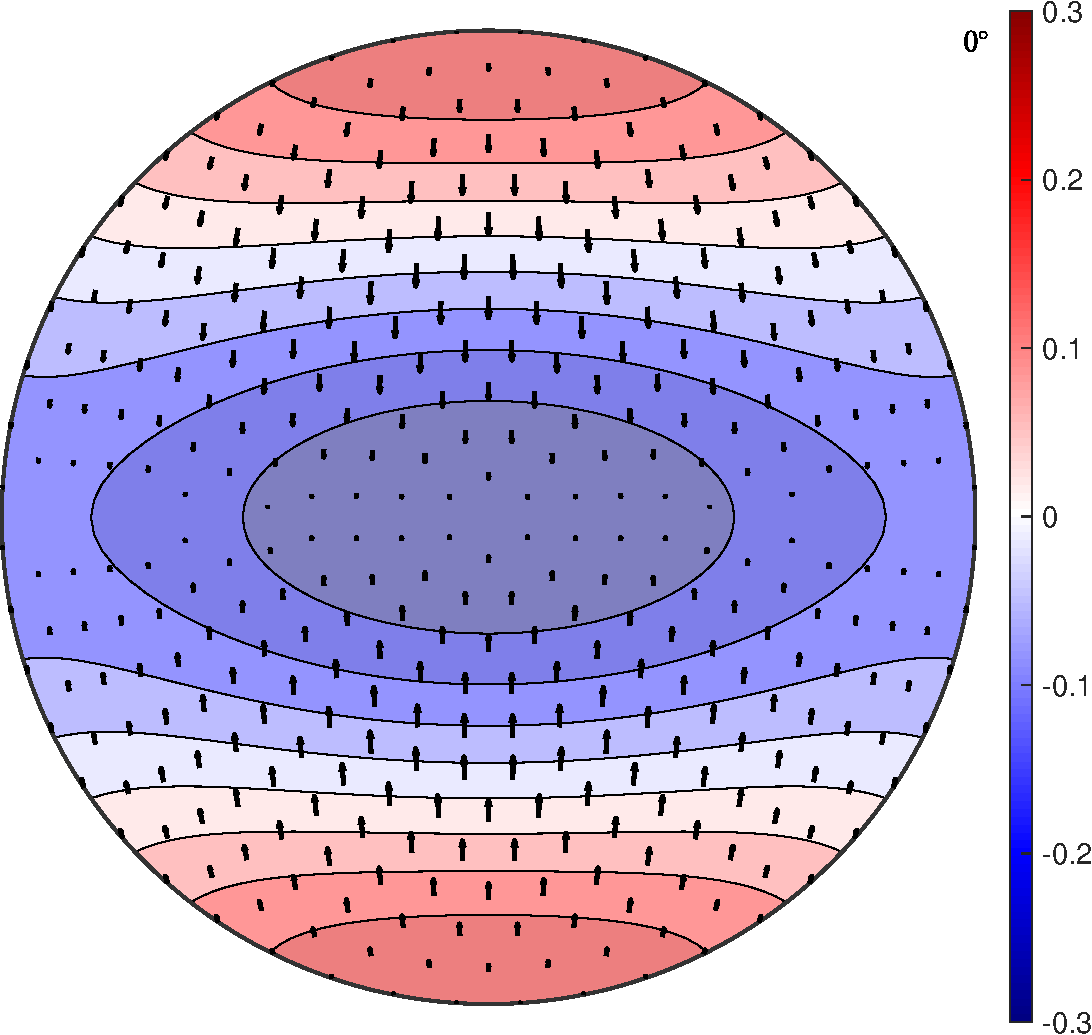
\includegraphics[height=0.46\textheight]{pic/Omega.pdf}

      \medskip
      
      \only<1>{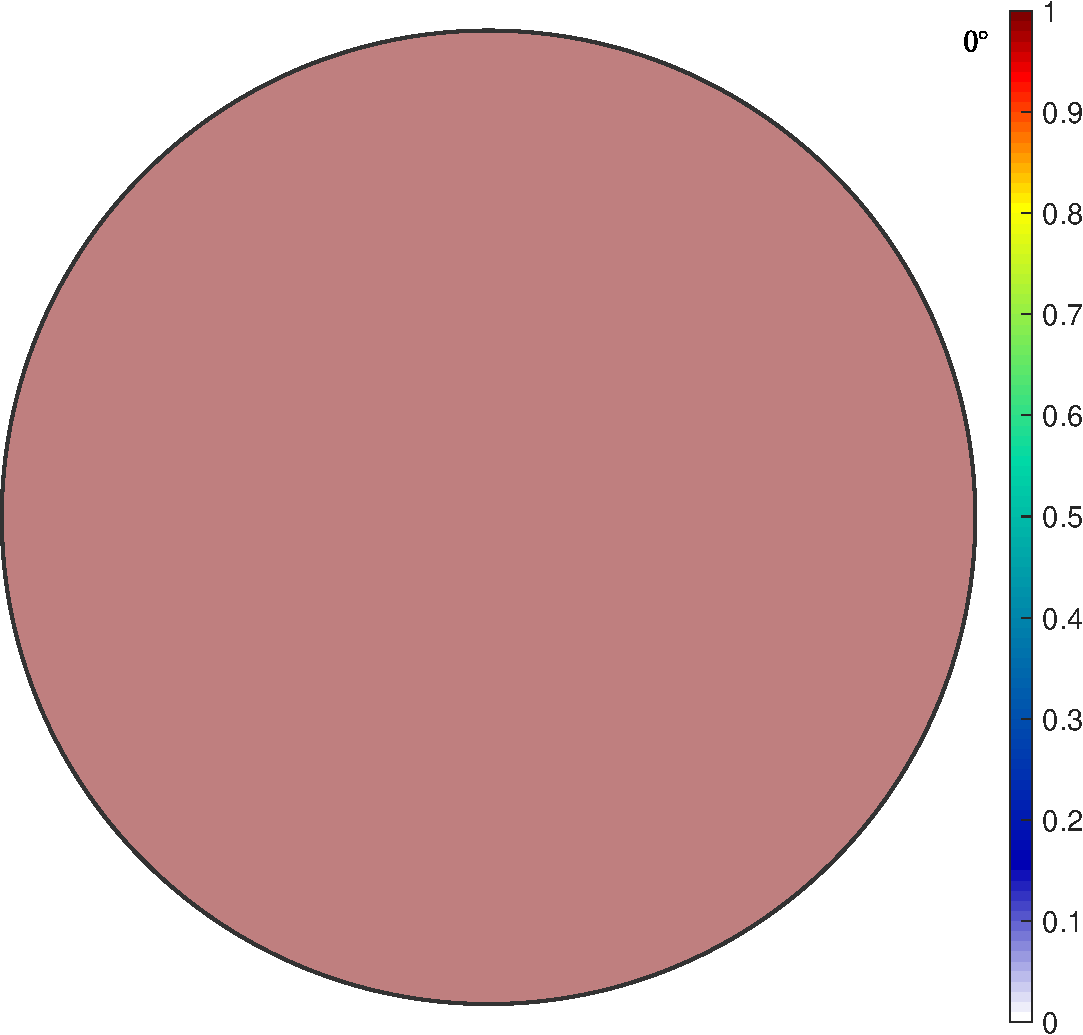
\includegraphics[height=0.46\textheight]{pic/odf0.pdf}}
      \only<2>{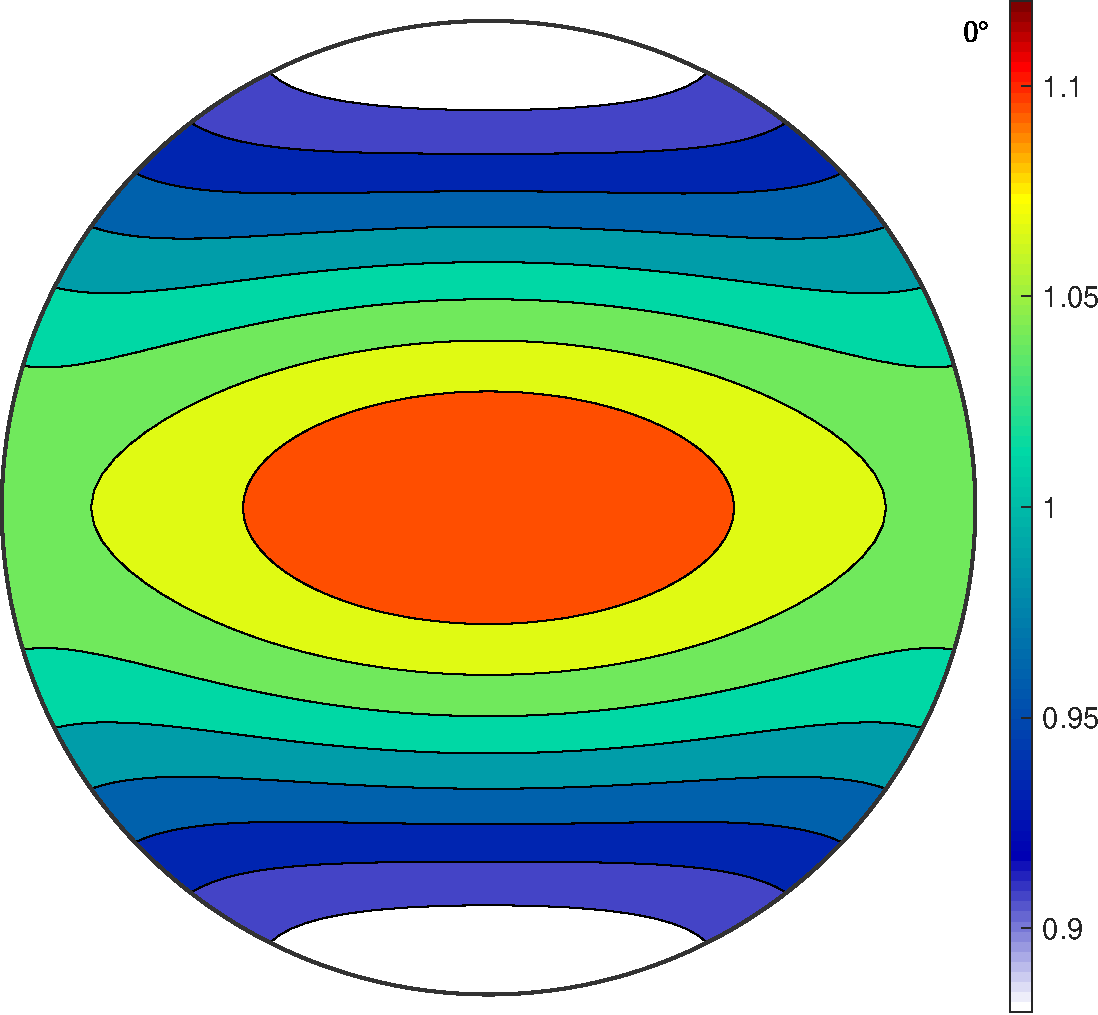
\includegraphics[height=0.46\textheight]{pic/odfE1.pdf}}
      \only<3>{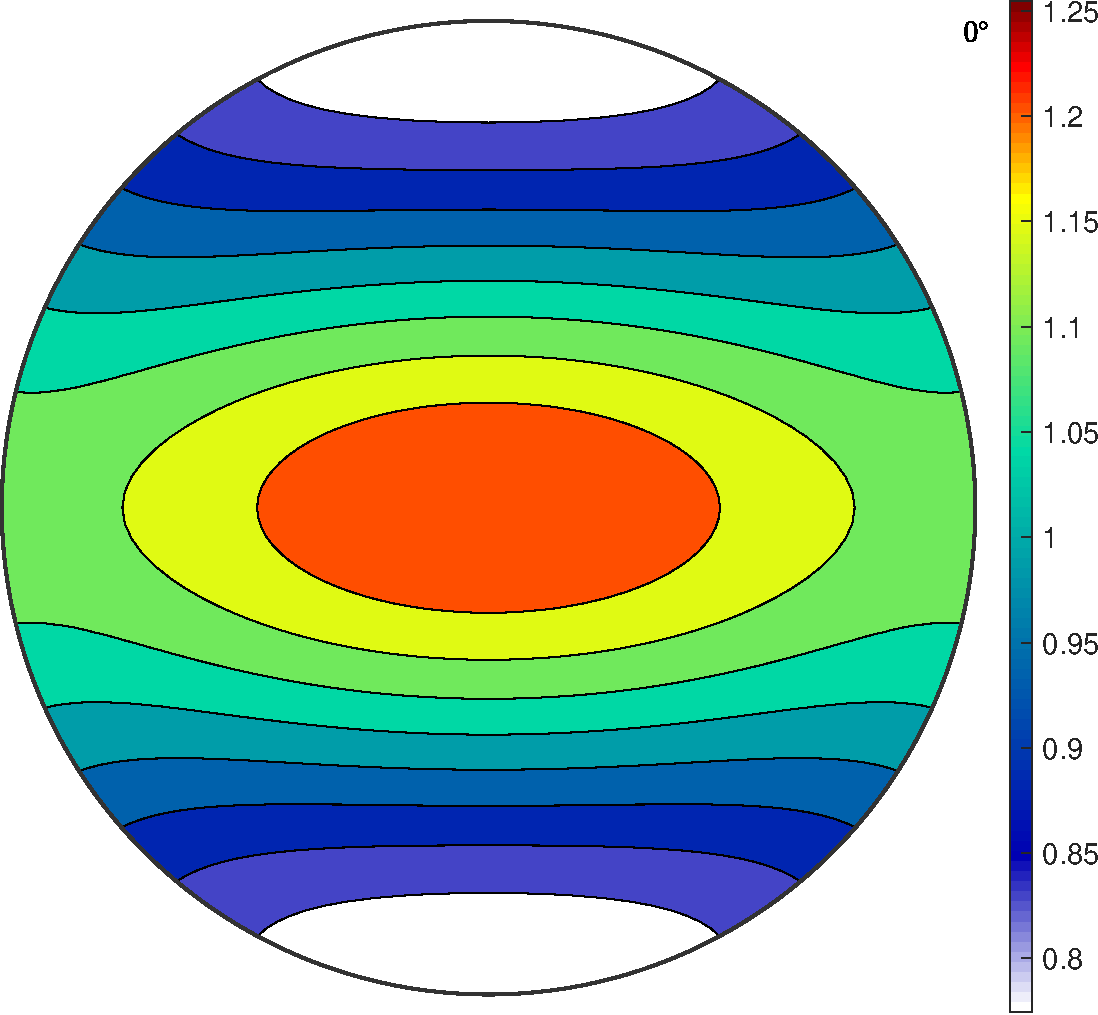
\includegraphics[height=0.46\textheight]{pic/odfE2.pdf}}
      \only<4>{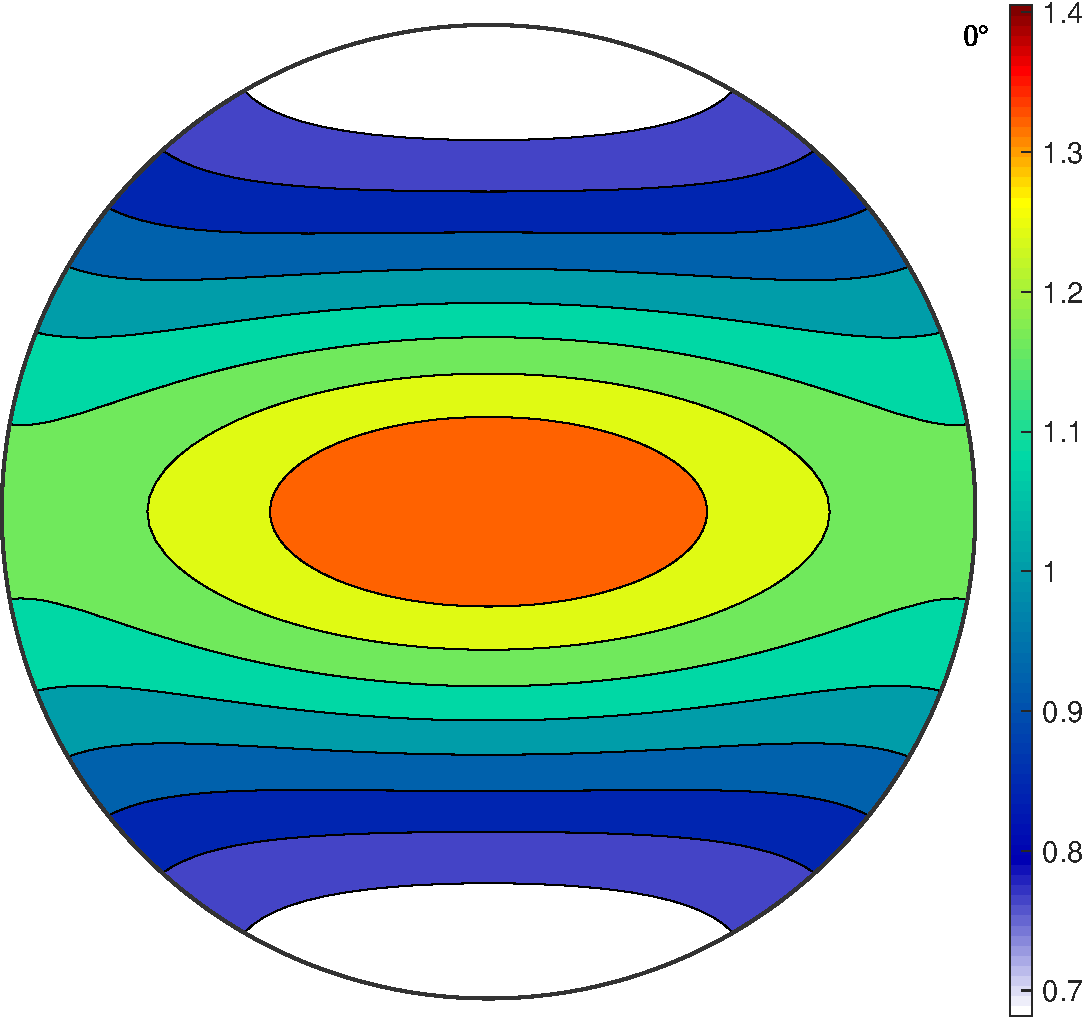
\includegraphics[height=0.46\textheight]{pic/odfE3.pdf}}
      \only<5>{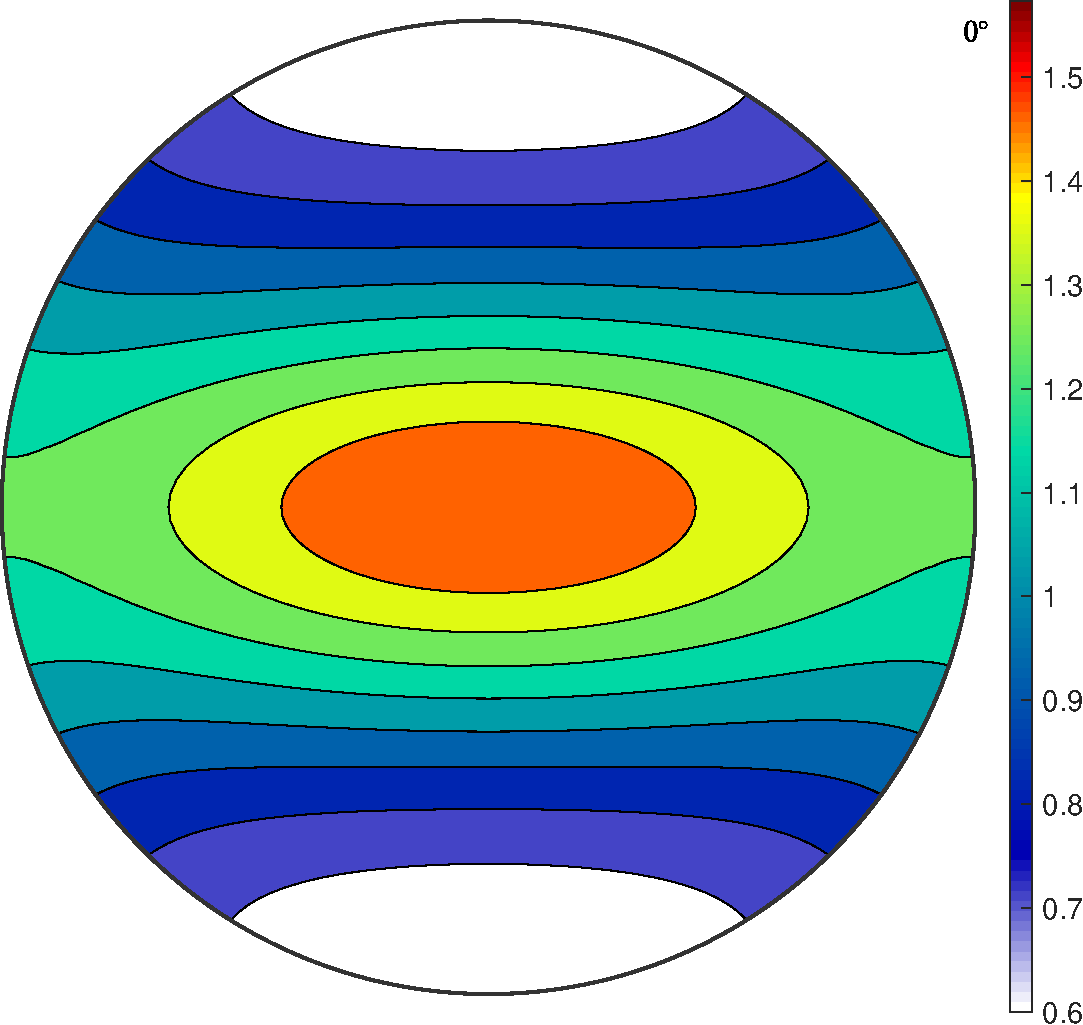
\includegraphics[height=0.46\textheight]{pic/odfE4.pdf}}
      \only<6>{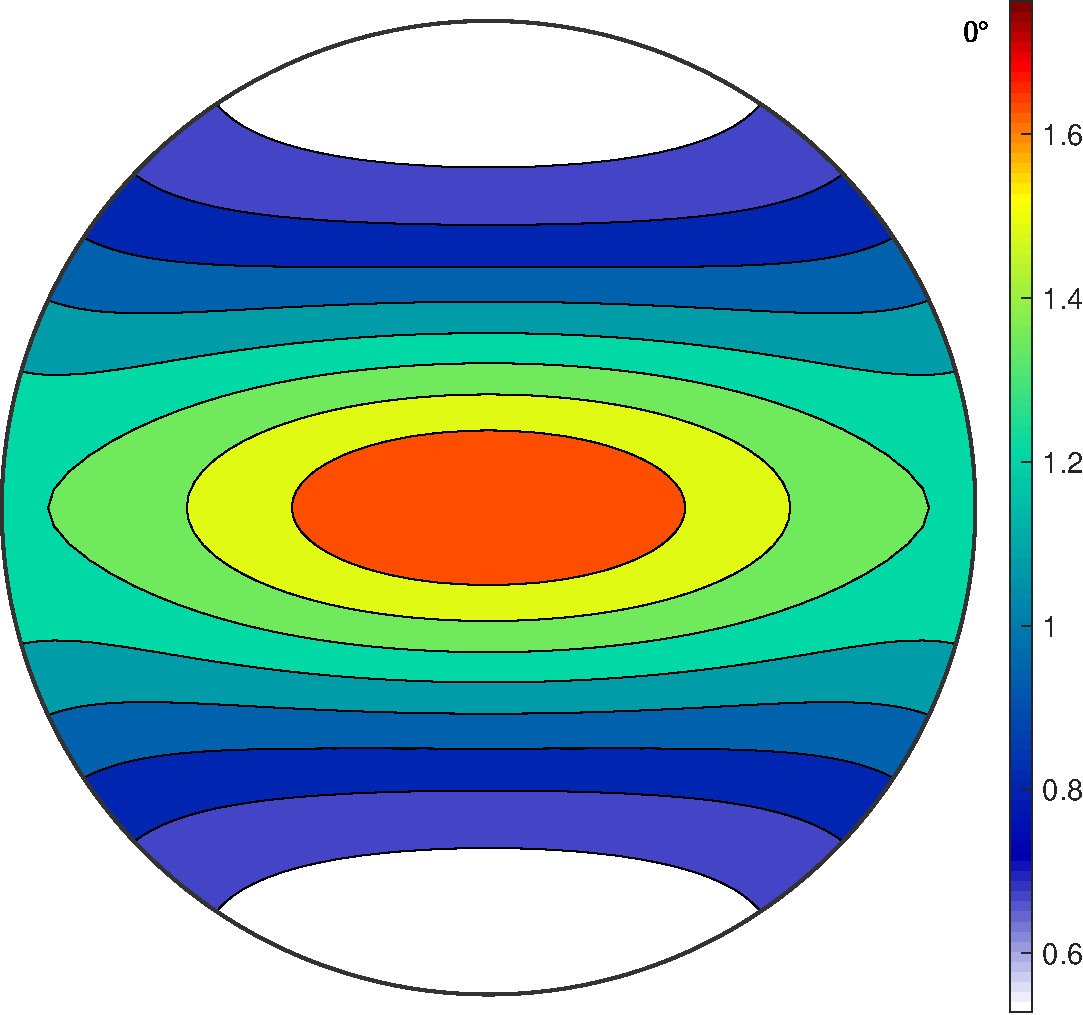
\includegraphics[height=0.46\textheight]{pic/odfE5.pdf}}
  \end{overlayarea}
\end{column}
\end{columns}
\end{frame}

% \begin{frame}[fragile]
%   \frametitle{Texture Evolution in Magnesium}

%   \begin{lstlisting}
% cs = crystalSymmetry.load('Mg-Magnesium.cif')
% odf = fibreODF(cs.cAxis, vector3d.Z);
% sScold = [slipSystem.basal(cs,1),...
%   slipSystem.prismatic2A(cs,66),...
%   slipSystem.pyramidalCA(cs,80),...
%   slipSystem.twinC1(cs,100)];

% sSwarm = [slipSystem.basal(cs,1),...
%   slipSystem.prismatic2A(cs,15),...
%   slipSystem.pyramidalCA(cs,10),...
%   slipSystem.twinC1(cs,100)];

% epsCold = 0.3 * strainTensor(diag([1 -0.6 -0.4]))
% epsWarm = 0.7 * strainTensor(diag([1 -0.5 -0.5]))

% % simulated an initial orientation distribution of 10000 grains
% ori = odf.discreteSample(10000);

% % apply the Taylor model
% [~,bCold,Wcold] = calcTaylor( inv(ori) .* epsCold, sScold);
% [~,bWarm,Wwarm] = calcTaylor( inv(ori) .* epsWarm, sSwarm);
%   \end{lstlisting}
% \end{frame}


% \begin{frame}[fragile]
%   \frametitle{Texture Evolution During Simple Shear}
% %
%     \begin{columns}
%       \begin{column}{0.73\textwidth}
%         \vspace{-1.2cm}
%         \begin{overlayarea}{\textwidth}{7.5cm}
%           \begin{lstlisting}[style=input]
% cs = crystalSymmetry('-3m');
% sS = [slipSystem({1,1,-2,0},{0,0,0,1},15,cs); ...
%   slipSystem({0,0,0,1},{1,0,-1,0},30,cs); ...
%   slipSystem({2,-1,-1,0},{0,1,-1,1},1,cs); ...
%   slipSystem({2,-1,-1,0},{-1,0,1,0},1,cs)];
% \end{lstlisting}
% \vspace{-0.2cm}
%           \begin{onlyenv}<2->
% \begin{lstlisting}[style=input]
% F = deformationGradientTensor.simpleShear(...
%      vector3d.Y, vector3d.X, 70*degree)
% \end{lstlisting}
%           \end{onlyenv}
%         \begin{onlyenv}<2|handout:0>
%           \vspace{-0.3cm}
% \begin{lstlisting}[style=output]
% F = /+deformationGradientTensor+/
%   rank: 2 (3 x 3)

%       1      0      0
%  2.7475      1      0
%       0      0      1
% \end{lstlisting}
%         \end{onlyenv}
% \vspace{-0.2cm}
%         \begin{onlyenv}<3->
% \begin{lstlisting}[style=input]
% L = logm(F) ./ nSteps
% W = L.antiSym, D = L.sym
% \end{lstlisting}
%         \end{onlyenv}
%         \begin{onlyenv}<3|handout:0>
%           \vspace{-0.3cm}
% \begin{lstlisting}[style=output]
% W = /+spinTensor+/         D = /+strainRateTensor+/
%   rank: 2 (3 x 3)            rank: 2 (3 x 3)

%  *10^-3                     *10^-3
%    0 -30   0                 0 30  0
%   30   0   0                30  0  0
%    0   0   0                 0  0  0
% \end{lstlisting}
%         \end{onlyenv}
% %
%         \begin{onlyenv}<4>
% \begin{lstlisting}[style=input]
% [~,~,W_Taylor] = calcTaylor(inv(ori) .* D, sS)
% \end{lstlisting}
%         \end{onlyenv}
%         \begin{onlyenv}<4|handout:0>
%           \vspace{-0.3cm}
% \begin{lstlisting}[style=output]
% W_Taylor = /+spinTensor+/
%   size   : 10000 x 1
%   rank   : 2 (3 x 3)
%   mineral: -3m1, X||a*, Y||b, Z||c*
% \end{lstlisting}
%         \end{onlyenv}
%         \begin{onlyenv}<5|handout:0>
% \begin{lstlisting}[style=input]
% for i = 1:nSteps
%   [~,~,W_Taylor] = calcTaylor(inv(ori) * D, sS)
%   ori = rotation(-W) .* ori
%         .* orientation(-W_Taylor)
% end
% \end{lstlisting}
%           \end{onlyenv}
%           \begin{onlyenv}<6|handout:0>
% \begin{lstlisting}[style=input]
% for i = 1:nSteps
%   [~,~,W_Taylor] = calcTaylor(inv(ori) * D, sS)
%   W_total = W + ori .* W_Taylor;
%   ori = rotation(-W_total) .* ori;
% end
% \end{lstlisting}
%           \end{onlyenv}
% \begin{onlyenv}<7->
% \begin{lstlisting}[style=input]
% for i = 1:nSteps
%   [~,~,W_Taylor] = calcTaylor(inv(ori) * D, sS)
%   W_total = inv(ori) * W + spin;
%   ori = ori .* orientation(-W_total);
% end
% \end{lstlisting}
% \end{onlyenv}
% \end{overlayarea}
% \end{column}
%   \begin{column}{0.24\textwidth}
%   \begin{overlayarea}{\textwidth}{8cm}
%     \vspace{-1cm}
%     \begin{onlyenv}<1-4|handout:0>
%       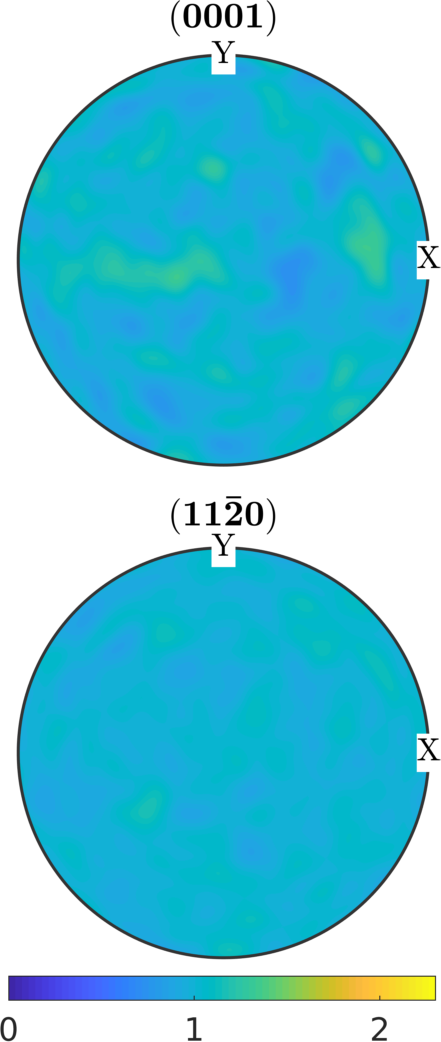
\includegraphics[width=\textwidth]{pic/quartz_0.png}
%     \end{onlyenv}
%     \begin{onlyenv}<5|handout:0>
%       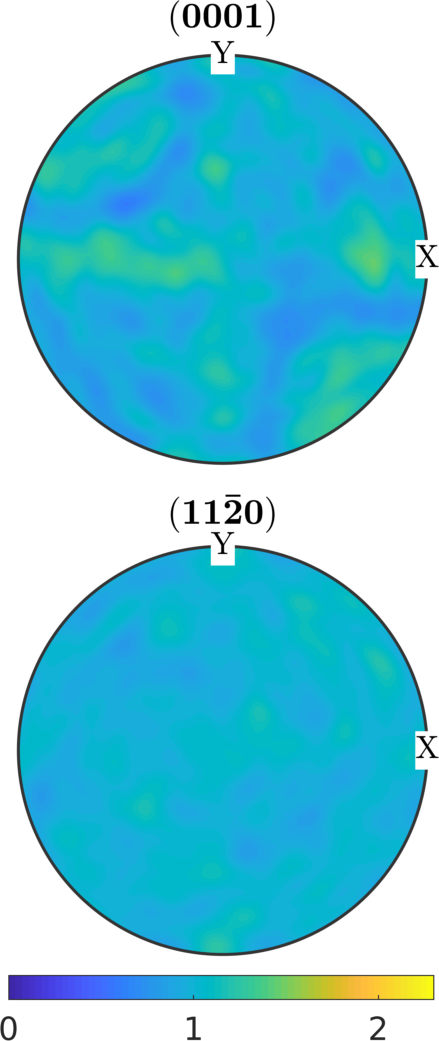
\includegraphics[width=\textwidth]{pic/quartz_1.png}
%     \end{onlyenv}
%     \begin{onlyenv}<6|handout:0>
%       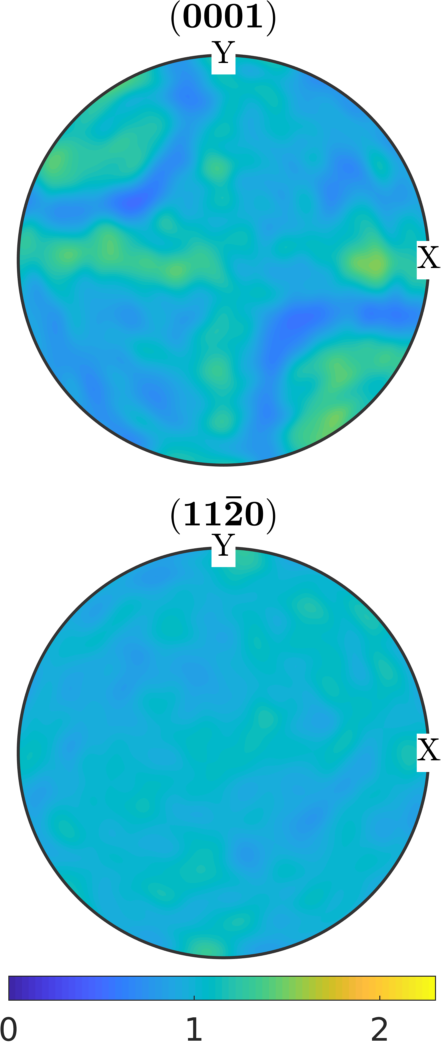
\includegraphics[width=\textwidth]{pic/quartz_2.png}
%     \end{onlyenv}
%     \begin{onlyenv}<7|handout:0>
%       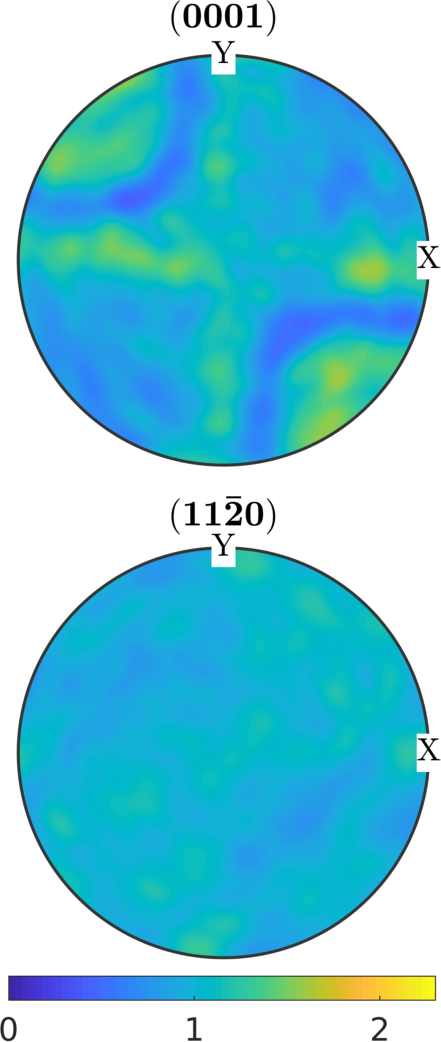
\includegraphics[width=\textwidth]{pic/quartz_3.png}
%     \end{onlyenv}
%     \begin{onlyenv}<8|handout:0>
%       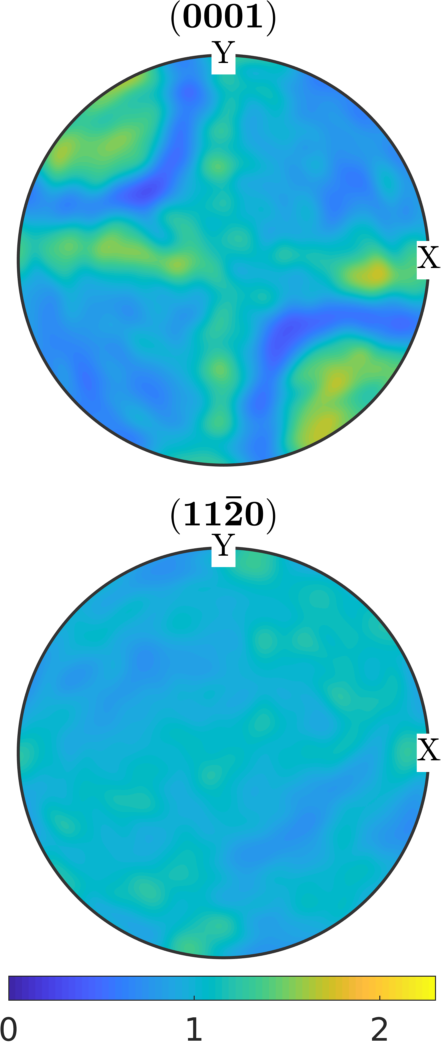
\includegraphics[width=\textwidth]{pic/quartz_4.png}
%     \end{onlyenv}
%     \begin{onlyenv}<9|handout:0>
%       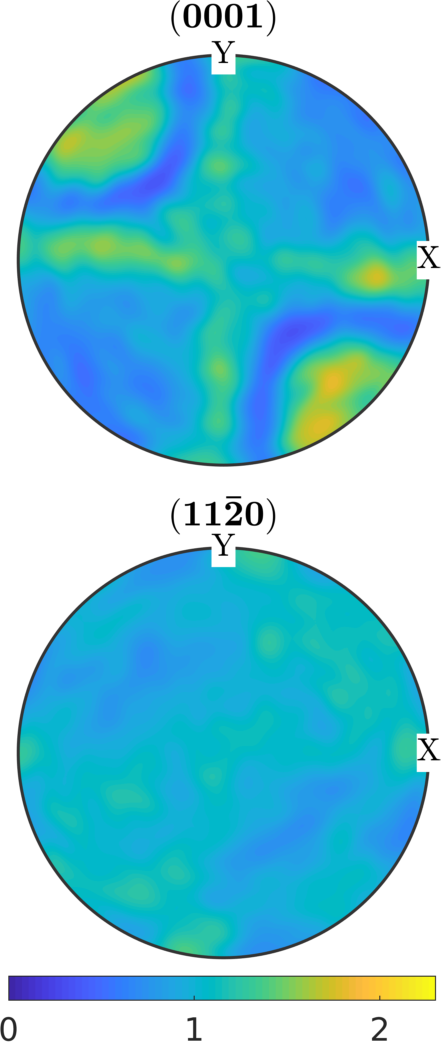
\includegraphics[width=\textwidth]{pic/quartz_5.png}
%     \end{onlyenv}
%     \begin{onlyenv}<10|handout:0>
%       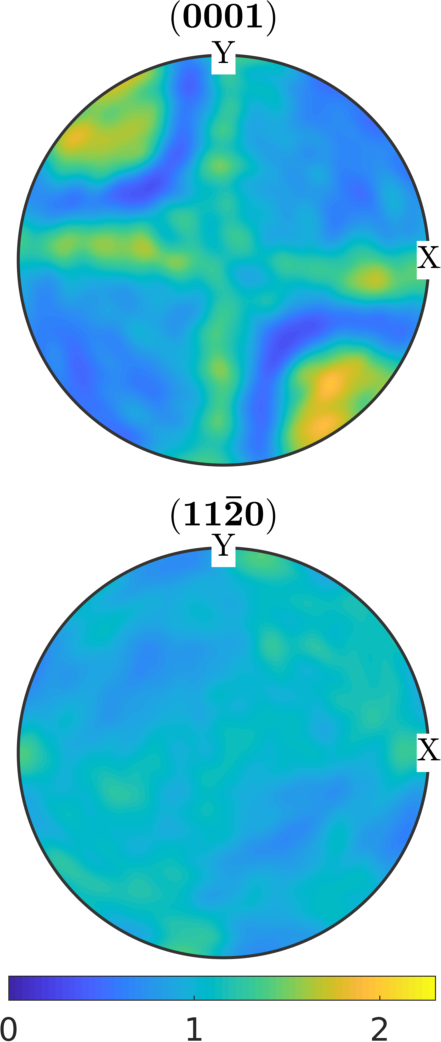
\includegraphics[width=\textwidth]{pic/quartz_6.png}
%     \end{onlyenv}
%     \begin{onlyenv}<11|handout:0>
%       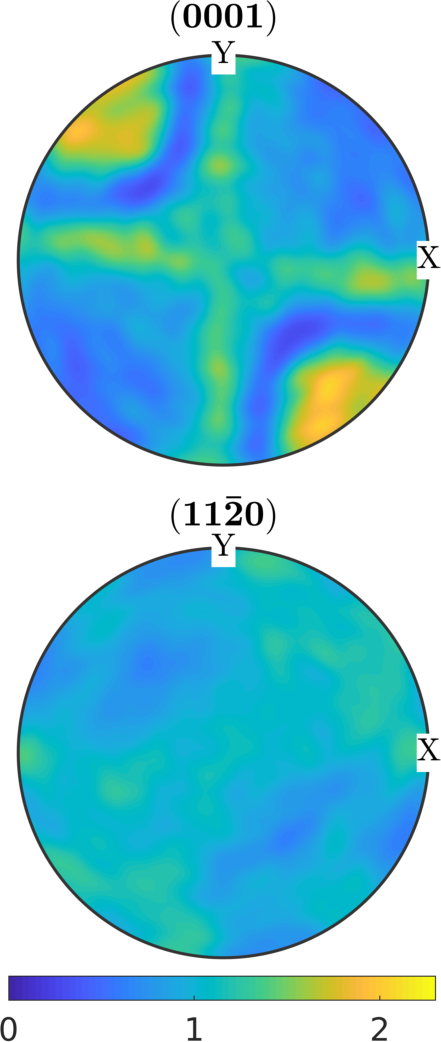
\includegraphics[width=\textwidth]{pic/quartz_7.png}
%     \end{onlyenv}
%     \begin{onlyenv}<12|handout:0>
%       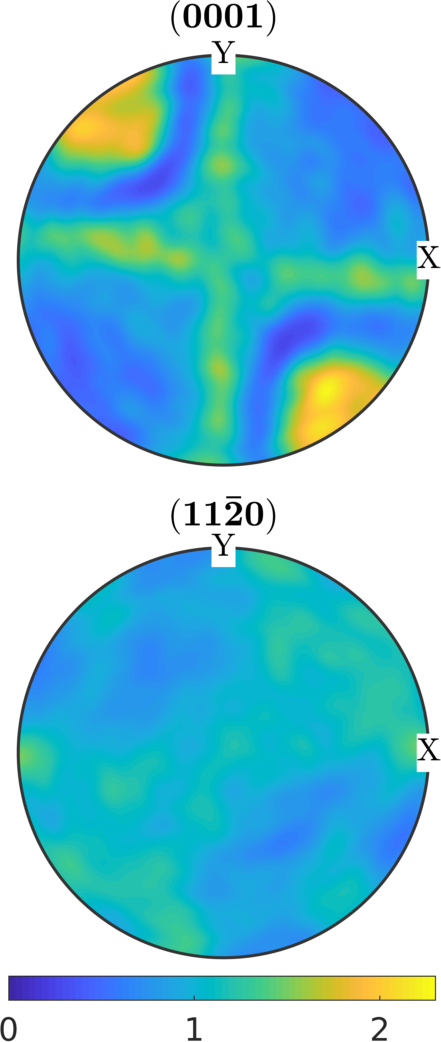
\includegraphics[width=\textwidth]{pic/quartz_8.png}
%     \end{onlyenv}
%     \begin{onlyenv}<13|handout:0>
%       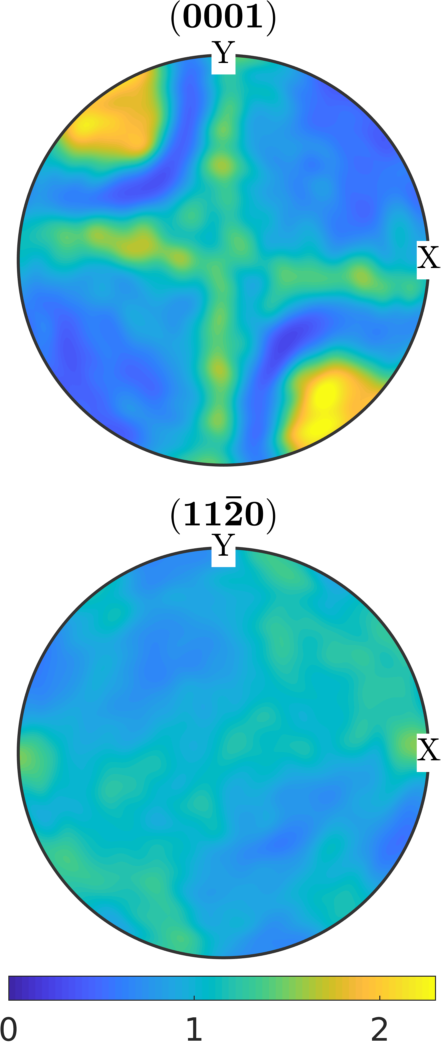
\includegraphics[width=\textwidth]{pic/quartz_9.png}
%     \end{onlyenv}
%     \begin{onlyenv}<14|handout:0>
%       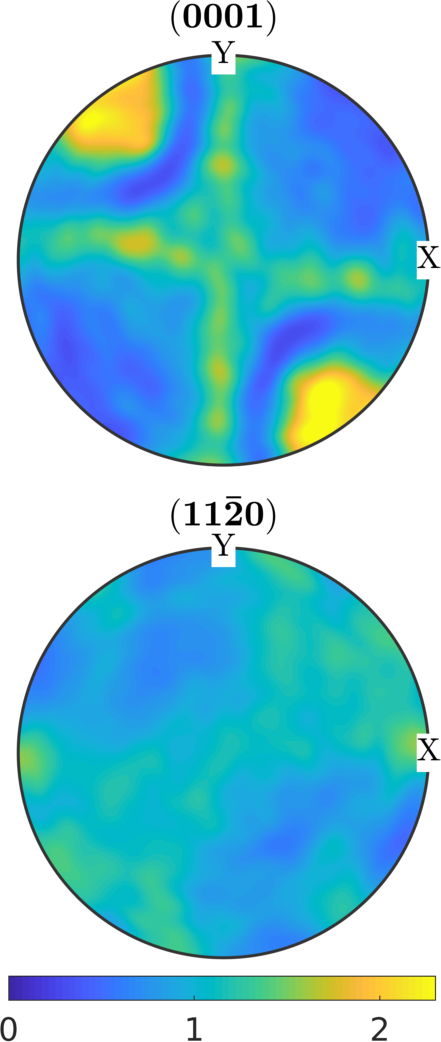
\includegraphics[width=\textwidth]{pic/quartz_10.png}
%     \end{onlyenv}
%     \begin{onlyenv}<15|handout:0>
%       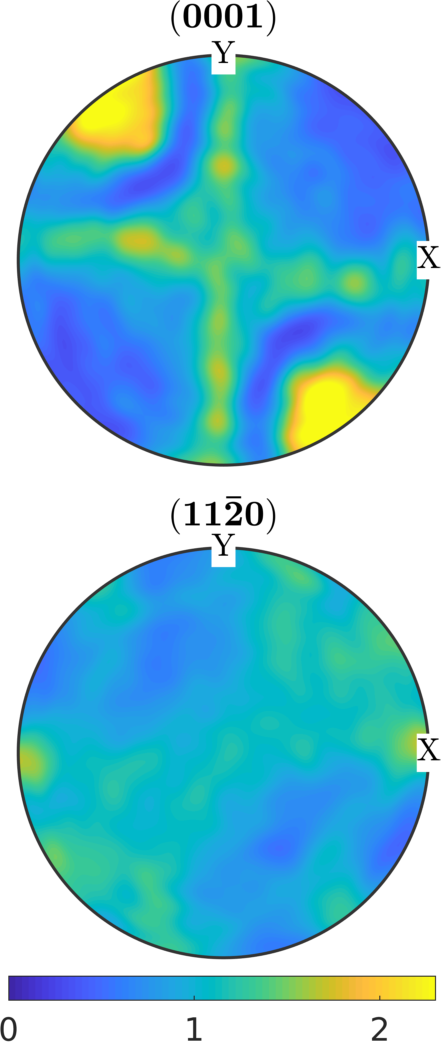
\includegraphics[width=\textwidth]{pic/quartz_11.png}
%     \end{onlyenv}
%     \begin{onlyenv}<16|handout:0>
%       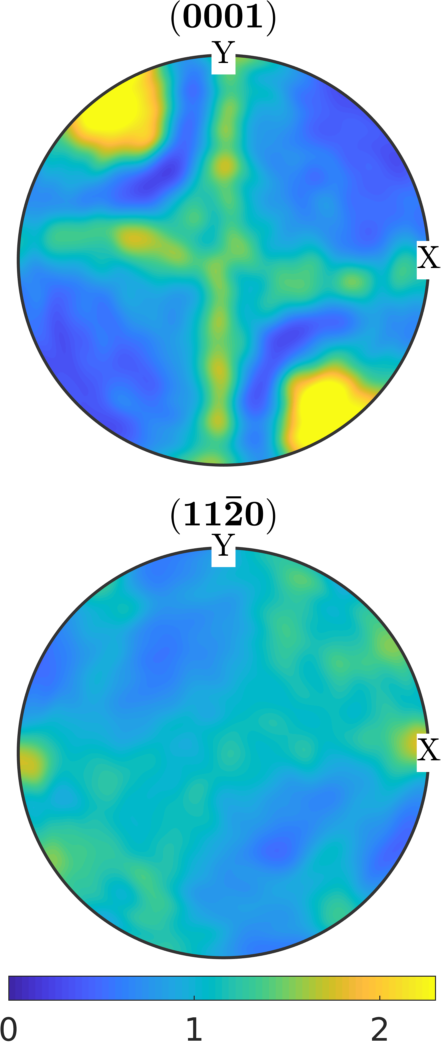
\includegraphics[width=\textwidth]{pic/quartz_12.png}
%     \end{onlyenv}
%     \begin{onlyenv}<17|handout:0>
%       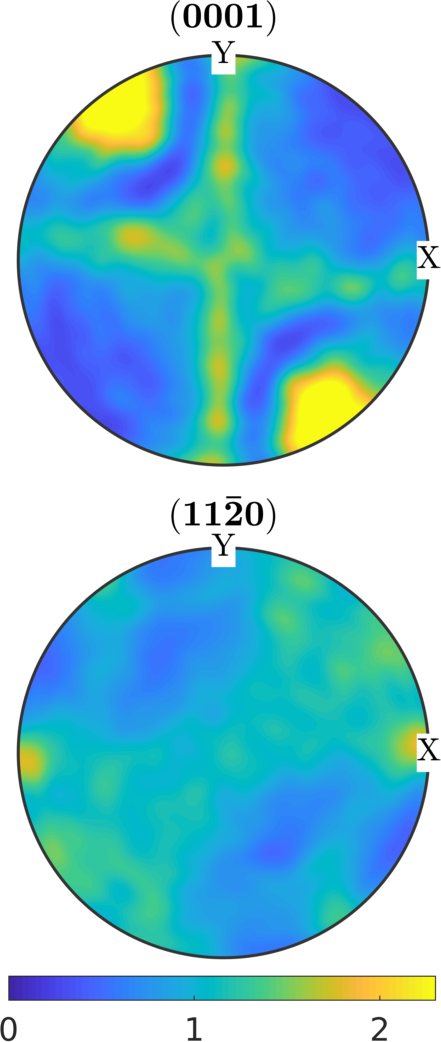
\includegraphics[width=\textwidth]{pic/quartz_13.png}
%     \end{onlyenv}
%     \begin{onlyenv}<18|handout:0>
%       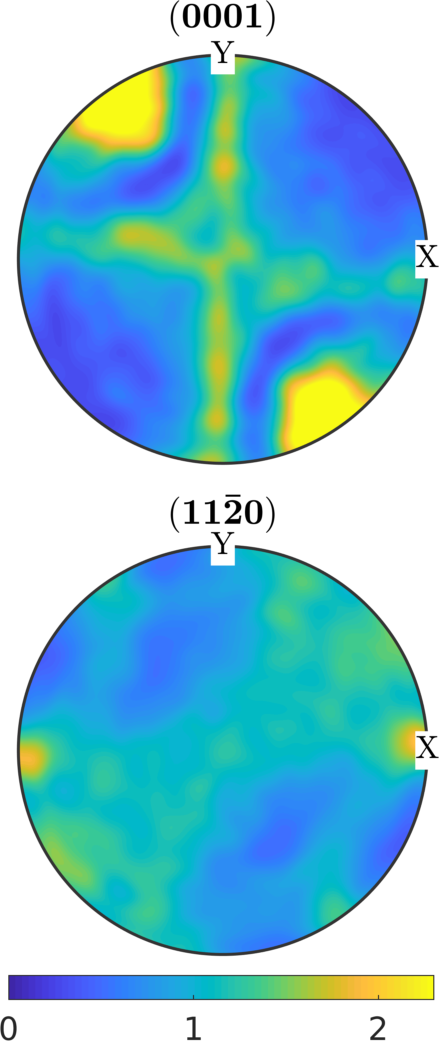
\includegraphics[width=\textwidth]{pic/quartz_14.png}
%     \end{onlyenv}
%     \begin{onlyenv}<19|handout:0>
%       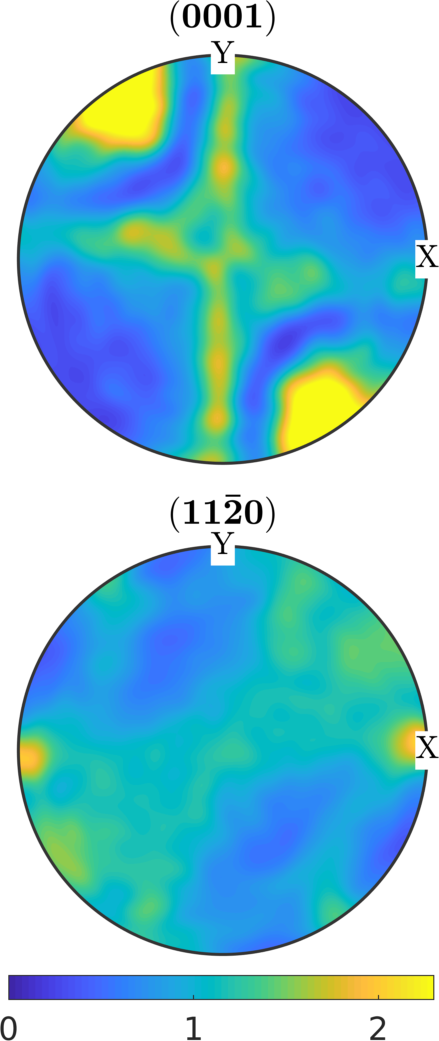
\includegraphics[width=\textwidth]{pic/quartz_15.png}
%     \end{onlyenv}
%     \begin{onlyenv}<20|handout:0>
%       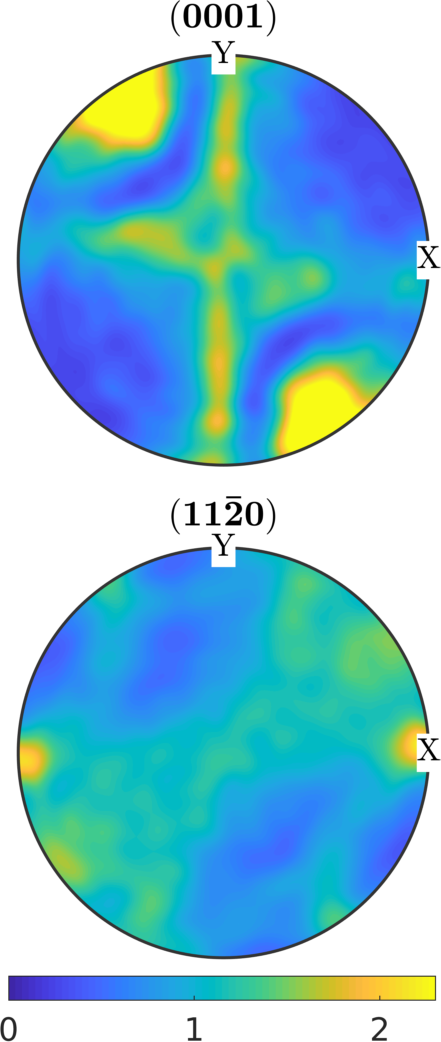
\includegraphics[width=\textwidth]{pic/quartz_16.png}
%     \end{onlyenv}
%     \begin{onlyenv}<21|handout:0>
%       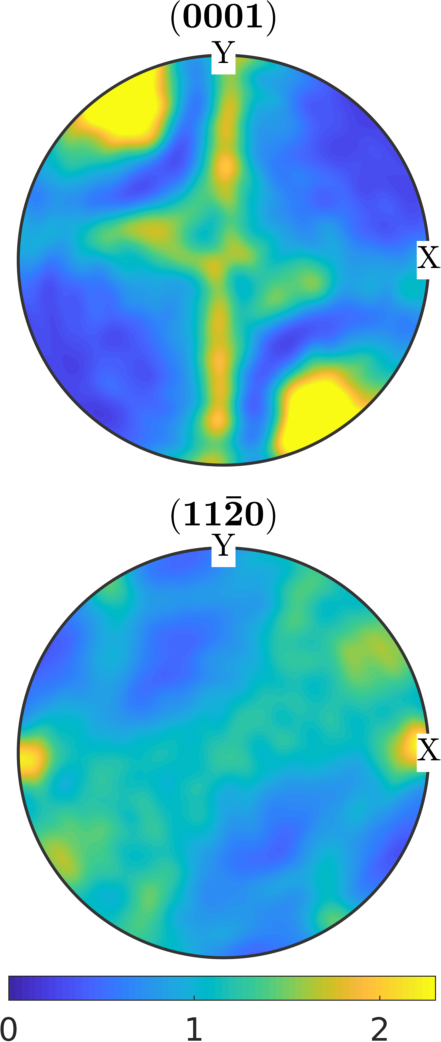
\includegraphics[width=\textwidth]{pic/quartz_17.png}
%     \end{onlyenv}
%     \begin{onlyenv}<22|handout:0>
%       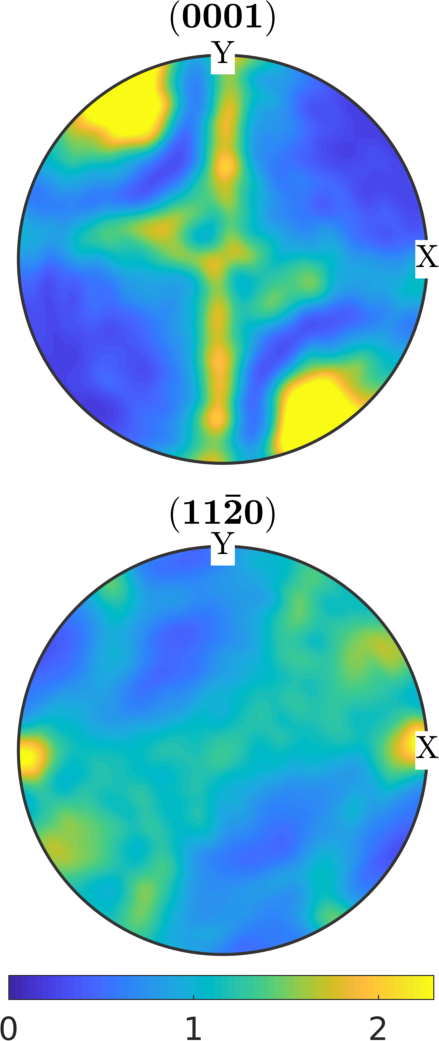
\includegraphics[width=\textwidth]{pic/quartz_18.png}
%     \end{onlyenv}
%     \begin{onlyenv}<23|handout:0>
%       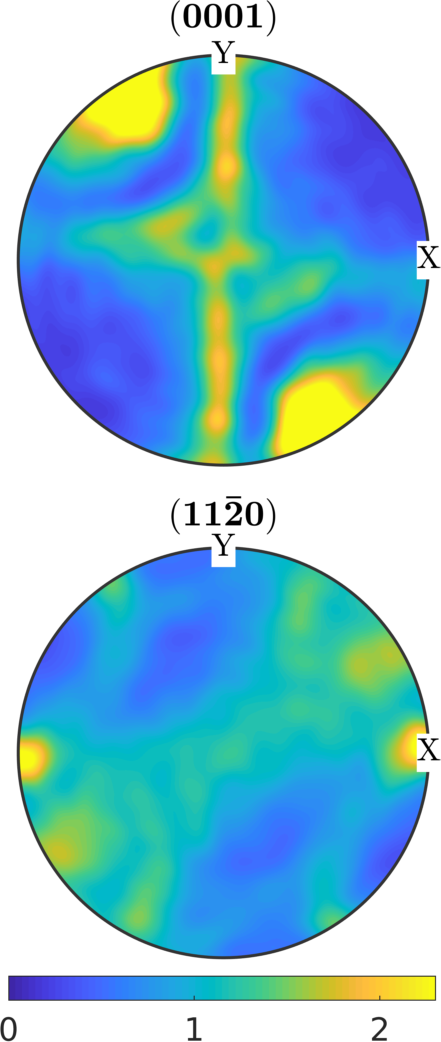
\includegraphics[width=\textwidth]{pic/quartz_19.png}
%     \end{onlyenv}
%     \begin{onlyenv}<24>
%       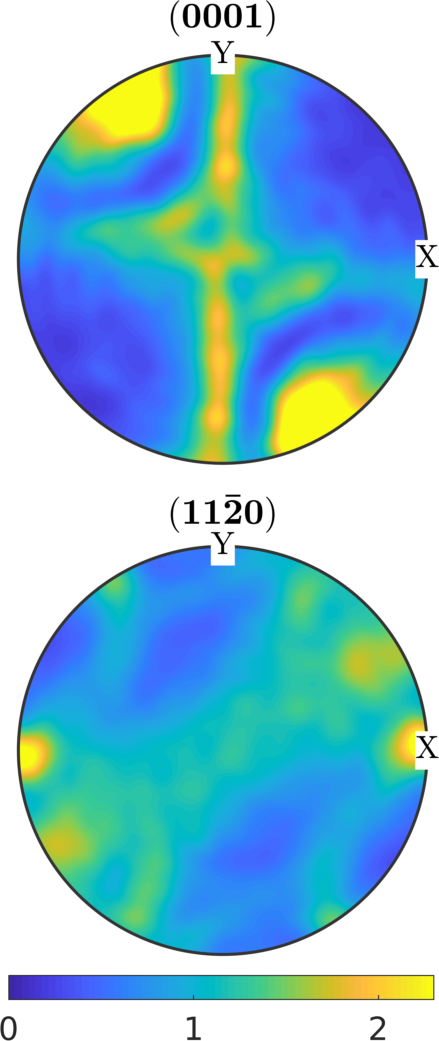
\includegraphics[width=\textwidth]{pic/quartz_20.png}
%     \end{onlyenv}
%   \end{overlayarea}
% \end{column}
% \end{columns}

% \end{frame}


% \begin{frame}[fragile]
%   \frametitle{Misc}
%   \vspace{-0.5cm}
%   \begin{overlayarea}{\textwidth}{8cm}

%       \begin{lstlisting}[style=input]
% epsGrain
% \end{lstlisting}
% \begin{onlyenv}<1>
%     \vspace{-0.3cm}
%   \begin{lstlisting}[style=output]
% epsGrain = /+strainTensor+/ (show methods, plot)
%   size   : 37 x 1
%   rank   : 2 (3 x 3)
%   mineral: fcc (432)
% \end{lstlisting}
% \end{onlyenv}
% \pause

%   \begin{lstlisting}[style=input]
% epsGrain(1)
% \end{lstlisting}
% \begin{onlyenv}<2>
%     \vspace{-0.3cm}
%     \begin{lstlisting}[style=output]
% ans = /+strainTensor+/ (show methods, plot)
%   rank   : 2 (3 x 3)
%   mineral: fcc (432)

%  *10^-2
%   57.35  -24.9 -70.07
%   -24.9 -20.11   7.41
%  -70.07   7.41 -37.24
% \end{lstlisting}
% \end{onlyenv}
% \pause
% \begin{lstlisting}[style=input]
% epsGrain{1,1}
% \end{lstlisting}
% \begin{onlyenv}<3>
%   \vspace{-0.3cm}
% \begin{lstlisting}[style=output]
% ans =
%     0.5735
%     0.7898
%    -0.2335
%     0.5767
%     0.1689
%     0.1850
%     0.7818
%    -0.1903
%    -0.2332
%     0.6518
%     0.1988
%     0.2005
%     0.1999
%    -0.2329
%     0.6348
%    -0.2345
%     0.1990
%    -0.2349
%     0.1993
% \end{lstlisting}
% \end{onlyenv}
% \end{overlayarea}
% \end{frame}


\begin{frame}[fragile]
  \frametitle{Geometrically Necessary Dislocations}

  \begin{overlayarea}{\textwidth}{\textheight}
    \begin{onlyenv}<1-2,4-10>
      \vspace{-0.3cm}
\begin{lstlisting}[style=input]
ebsd = loadEBSD('DC06_2undef.ang')
\end{lstlisting}
    \end{onlyenv}
%
    \begin{onlyenv}<1|handout:0>
      \vspace{-0.3cm}
\begin{lstlisting}[style=output]
ebsd = /+EBSD+/

 Phase  Orientations       Mineral  Symmetry
     0          5123  Iron (Alpha)       432

 Properties: ci, fit, iq, sem_signal, x, y, grainId
 Scan unit : um
 Grid size : 51 x 101
\end{lstlisting}
%\vspace{-0.3cm}
      \begin{center}
        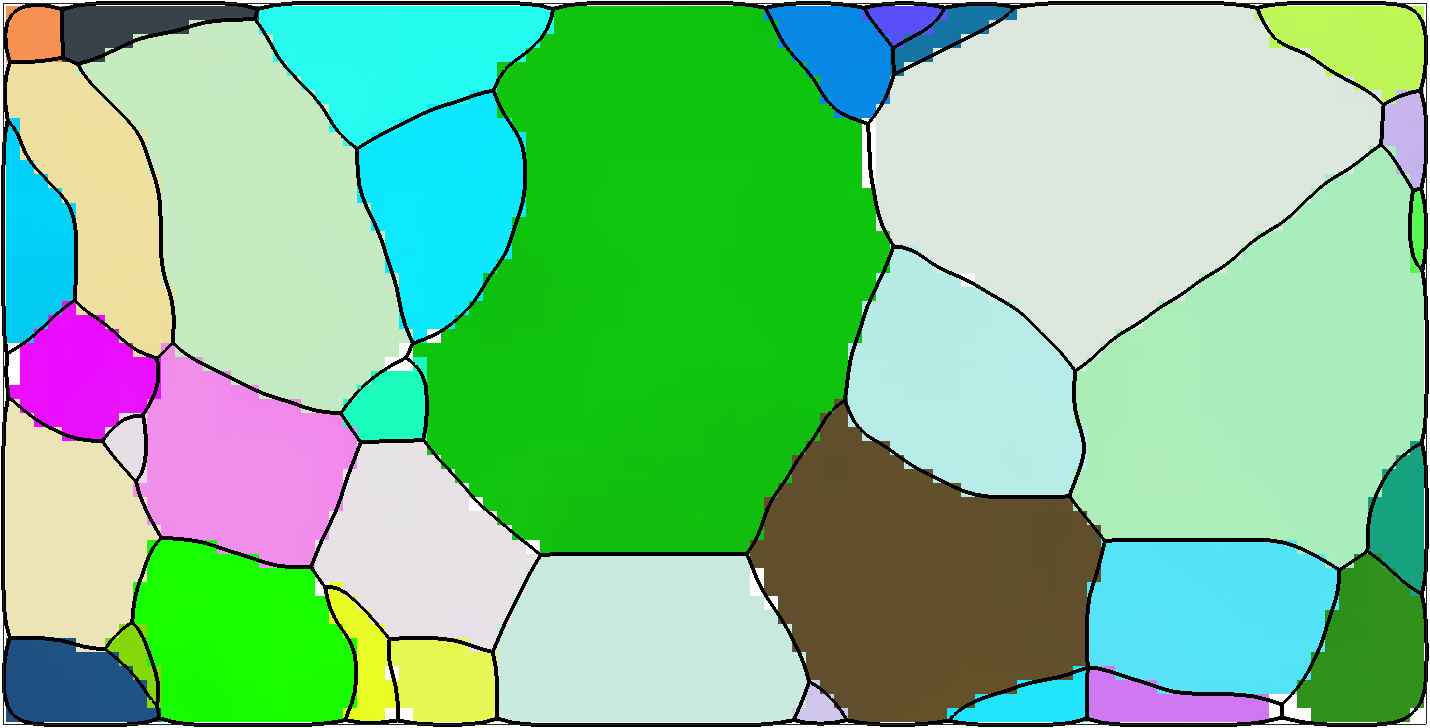
\includegraphics[width=0.5\textwidth]{pic/ebsd.png}
      \end{center}
    \end{onlyenv}
    \begin{onlyenv}<2,4-10>
      \vspace{-0.35cm}
\begin{lstlisting}[style=input]
kappa = ebsd.curvature
\end{lstlisting}
    \end{onlyenv}
    \begin{onlyenv}<2|handout:0>
      \vspace{-0.3cm}
\begin{lstlisting}[style=output]
kappa = /+curvatureTensor+/ (xyz)
  size: 51 x 101
  unit: 1/um
  rank: 2 (3 x 3)
\end{lstlisting}

\begin{lstlisting}[style=input]
kappa(2,3)
\end{lstlisting}
      \vspace{-0.3cm}
\begin{lstlisting}[style=output]
ans = /+curvatureTensor+/ (xyz)
  unit: 1/um
  rank: 2 (3 x 3)

 *10^-5
  -7.262  12.678     NaN
 -18.454  27.836     NaN
 -20.467  25.478     NaN
\end{lstlisting}
    \end{onlyenv}
    \begin{onlyenv}<3|handout:0>
      \vspace{-0.3cm}
\begin{lstlisting}[style=input]
plot(ebsd,kappa{1,1})
\end{lstlisting}
      \vspace{-0.2cm}
  \begin{center}
    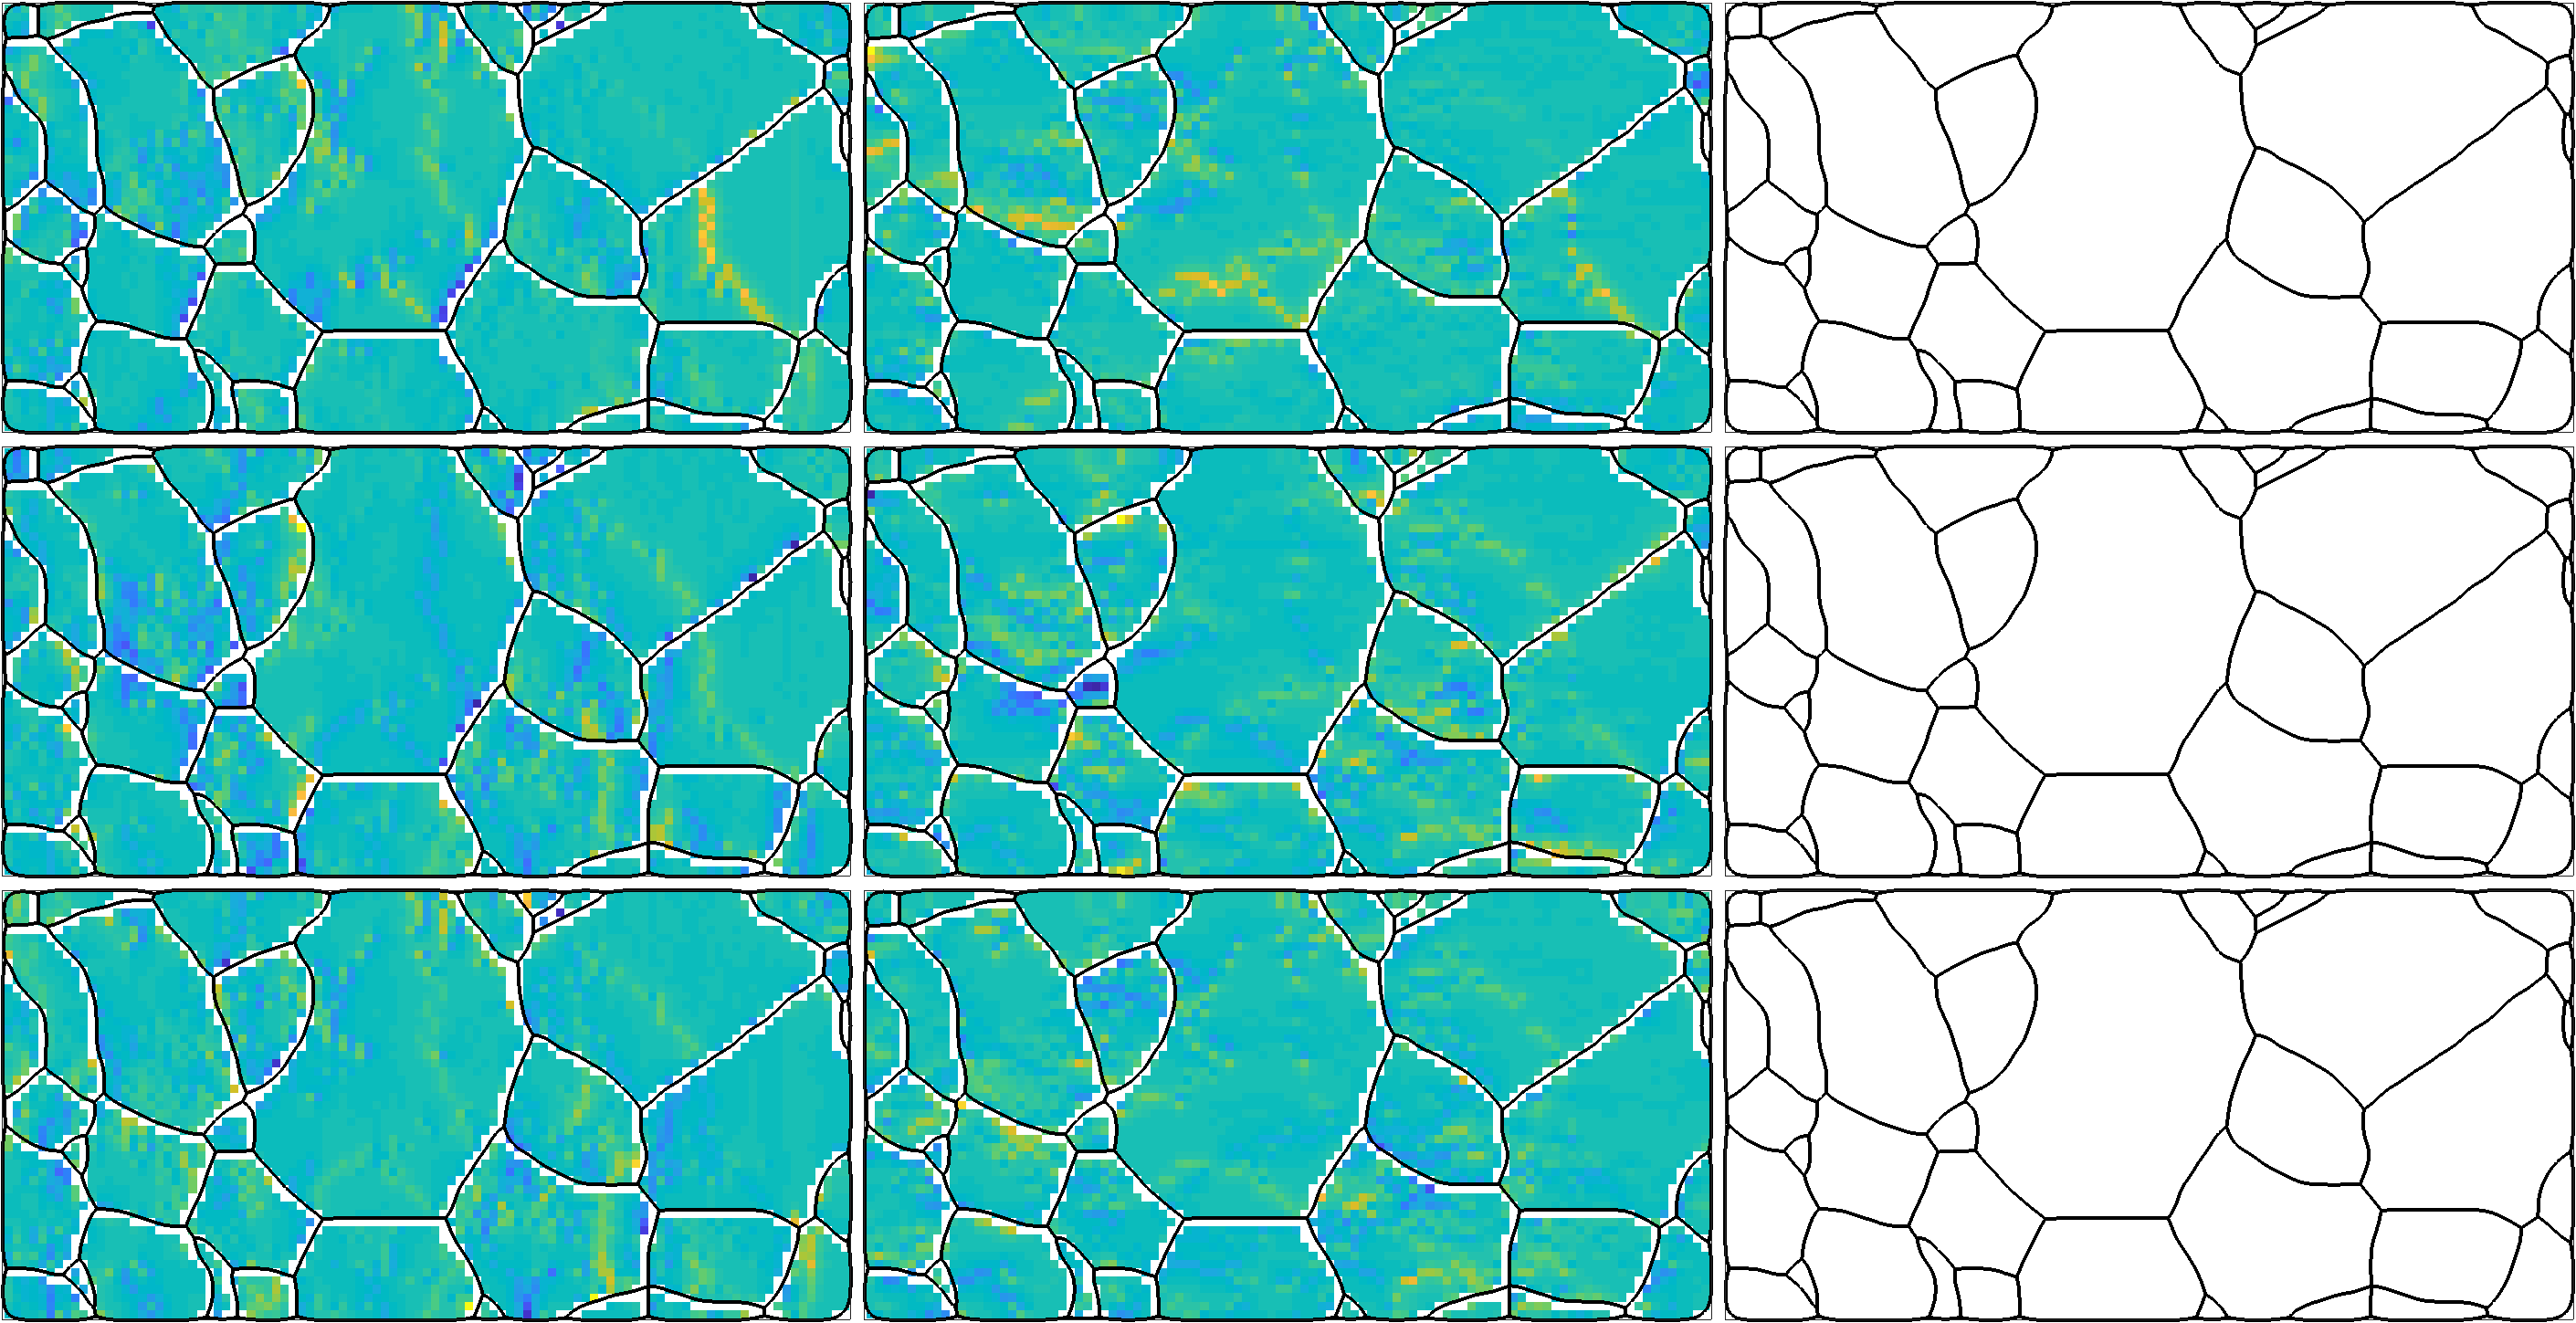
\includegraphics[width=0.87\textwidth]{pic/curvatureIncomplete}
  \end{center}
  \end{onlyenv}
  \begin{onlyenv}<4-10>
    \vspace{-0.35cm}
   \begin{lstlisting}[style=input]
alpha = kappa.dislocationDensity
\end{lstlisting}
\end{onlyenv}
\begin{onlyenv}<4|handout:0>
\vspace{-0.4cm}
\begin{lstlisting}[style=output]
alpha = /+dislocationDensityTensor+/ (xyz)
  size: 51 x 101
  unit: 1/um
  rank: 2 (3 x 3)
\end{lstlisting}
   \begin{lstlisting}[style=input]
alpha(2,3)
\end{lstlisting}
\vspace{-0.4cm}
\begin{lstlisting}[style=output]
ans = /+dislocationDensityTensor+/ (xyz)
  unit: 1/um
  rank: 2 (3 x 3)

 *10^-5
     NaN -18.454 -20.467
  12.678     NaN  25.478
     NaN     NaN -20.574
\end{lstlisting}
\end{onlyenv}
  \begin{onlyenv}<5-10>
    \vspace{-0.35cm}
\begin{lstlisting}[style=input]
dS = dislocationSystem.bcc(ebsd.CS)
\end{lstlisting}
\end{onlyenv}
\begin{onlyenv}<5|handout:0>
\vspace{-0.3cm}
\begin{lstlisting}[style=output]
dS = /+dislocationSystem+/ (/+Iron (alpha)+/)

 edge dislocations : 48 x 1
 Burgers vector  line vector  energy
     [ 1 -1  1]   [-2 -1  1]       2
     [-1  1  1]   [ 0  1 -1]       2
     [-1  1  1]   [-1  4 -5]       2

 screw dislocations: 4 x 1
 Burgers vector  energy
     [-1 -1 -1]       1
     [ 1 -1  1]       1
     [-1  1  1]       1
     [ 1  1 -1]       1
\end{lstlisting}
\end{onlyenv}
  \begin{onlyenv}<6>
    \vspace{-0.35cm}
\begin{lstlisting}[style=input]
dS(1).tensor
\end{lstlisting}
\end{onlyenv}
\begin{onlyenv}<6|handout:0>
\vspace{-0.4cm}
\begin{lstlisting}[style=output]
ans = /+dislocationDensityTensor+/ (/*Iron (Alpha)*/)
  unit   : au
  rank   : 2 (3 x 3)

 -1.1717 -0.5858  0.5858
  1.1717  0.5858 -0.5858
 -1.1717 -0.5858  0.5858
\end{lstlisting}
\end{onlyenv}
  \begin{onlyenv}<7-10>
    \vspace{-0.35cm}
\begin{lstlisting}[style=input]
dSSample = ebsd.orientations * dS
\end{lstlisting}
\end{onlyenv}
\begin{onlyenv}<7|handout:0>
\vspace{-0.3cm}
\begin{lstlisting}[style=output]
dSSample = /+dislocationSystem+/ (xyz)
 edge dislocations : 5123 x 48
 screw dislocations: 5123 x 4
\end{lstlisting}
\end{onlyenv}
  \begin{onlyenv}<8-10>
    \vspace{-0.3cm}
\begin{lstlisting}[style=input]
[rho,factor] = kappa.fitDislocationSystems(dSSample);
\end{lstlisting}
\end{onlyenv}
  \begin{onlyenv}<9-10>
    \vspace{-0.35cm}
\begin{lstlisting}[style=input]
alpha = sum(dSSample.tensor .* rho,2)
\end{lstlisting}
\end{onlyenv}
\begin{onlyenv}<9>
\begin{lstlisting}[style=input]
alpha(2,3)
\end{lstlisting}
\vspace{-0.4cm}
\begin{lstlisting}[style=output]
ans = /+dislocationDensityTensor+/ (xyz)
  unit: 1/um
  rank: 2 (3 x 3)

 *10^-5
 -28.855 -18.454 -20.467
  12.678   6.243  25.478
  -1.337  -1.989 -20.574
\end{lstlisting}
\end{onlyenv}
\begin{onlyenv}<10>
  \vspace{-0.35cm}
\begin{lstlisting}[style=input]
kappa = alpha.curvature
\end{lstlisting}
\end{onlyenv}
\begin{onlyenv}<10|handout:0>
\vspace{-0.4cm}
\begin{lstlisting}[style=output]
kappa = /+curvatureTensor+/ (xyz)
  size: 51 x 101
  unit: 1/um
  rank: 2 (3 x 3)
\end{lstlisting}
\end{onlyenv}
    \begin{onlyenv}<11>
      \vspace{-0.3cm}
\begin{lstlisting}[style=input]
plot(ebsd,kappa{1,1})
\end{lstlisting}
      \vspace{-0.5cm}
  \begin{center}
    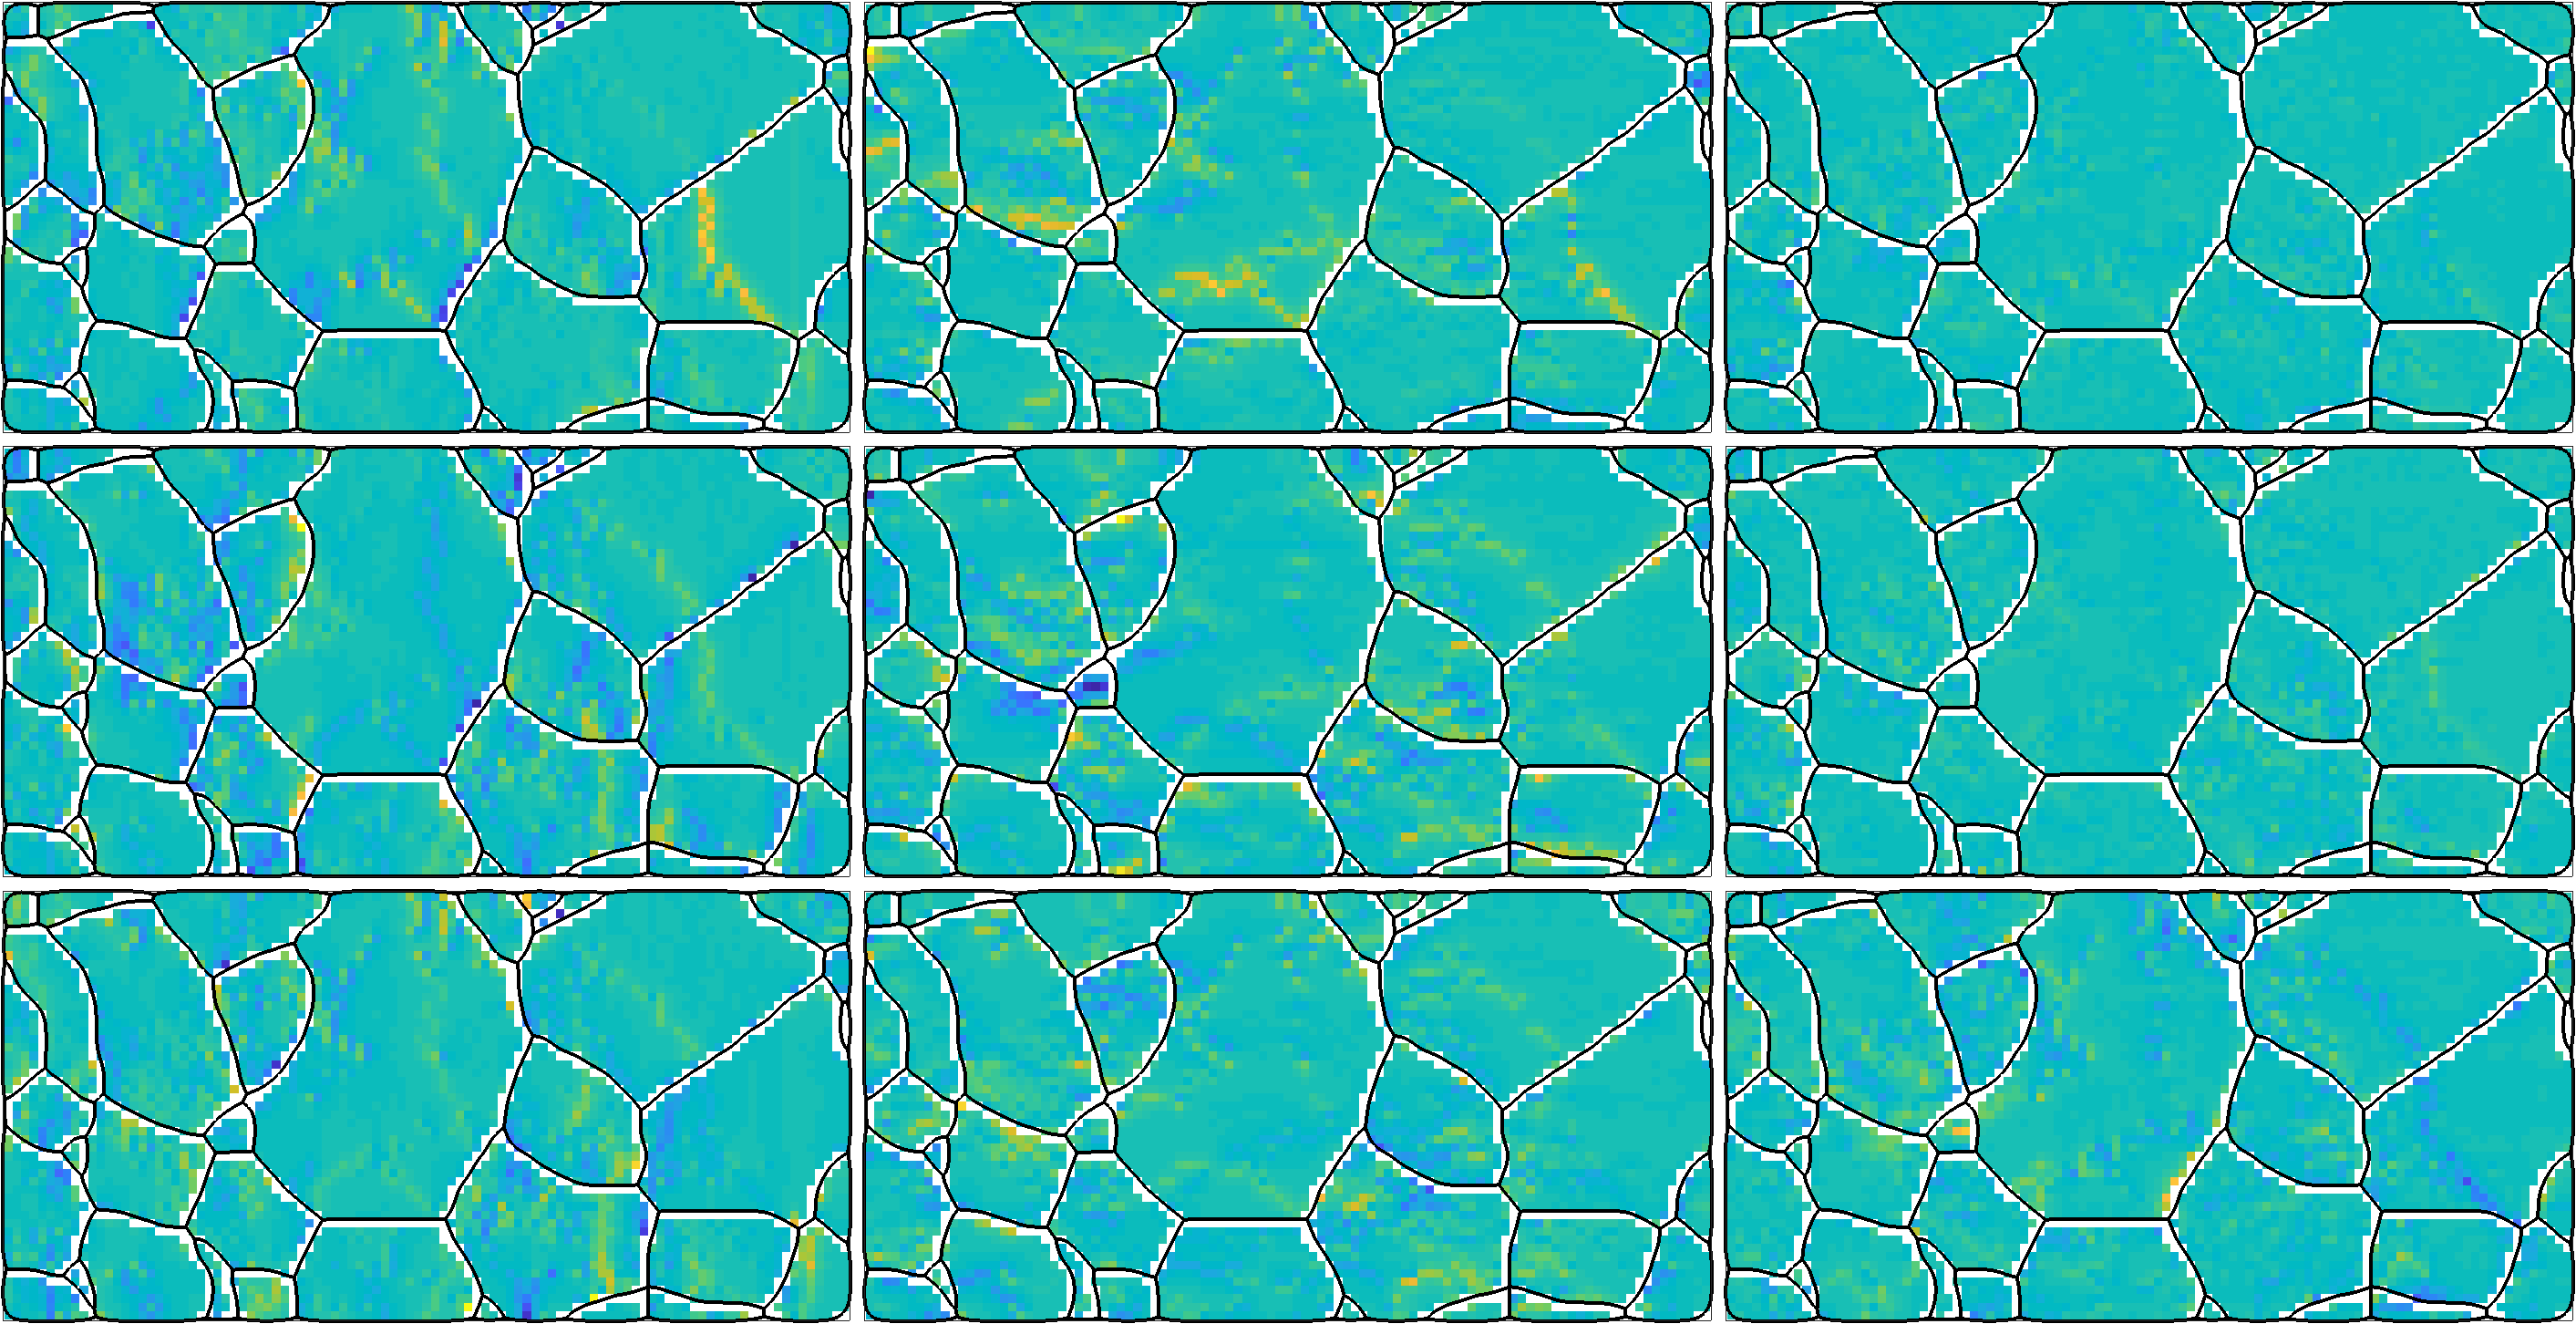
\includegraphics[width=0.87\textwidth]{pic/curvatureComplete}
  \end{center}
  \end{onlyenv}
      \begin{onlyenv}<12>
      \vspace{-0.3cm}
\begin{lstlisting}[style=input]
plot(ebsd,factor * sum(abs(rho .* dSSample.u),2))
\end{lstlisting}
      \vspace{-0.5cm}
  \begin{center}
    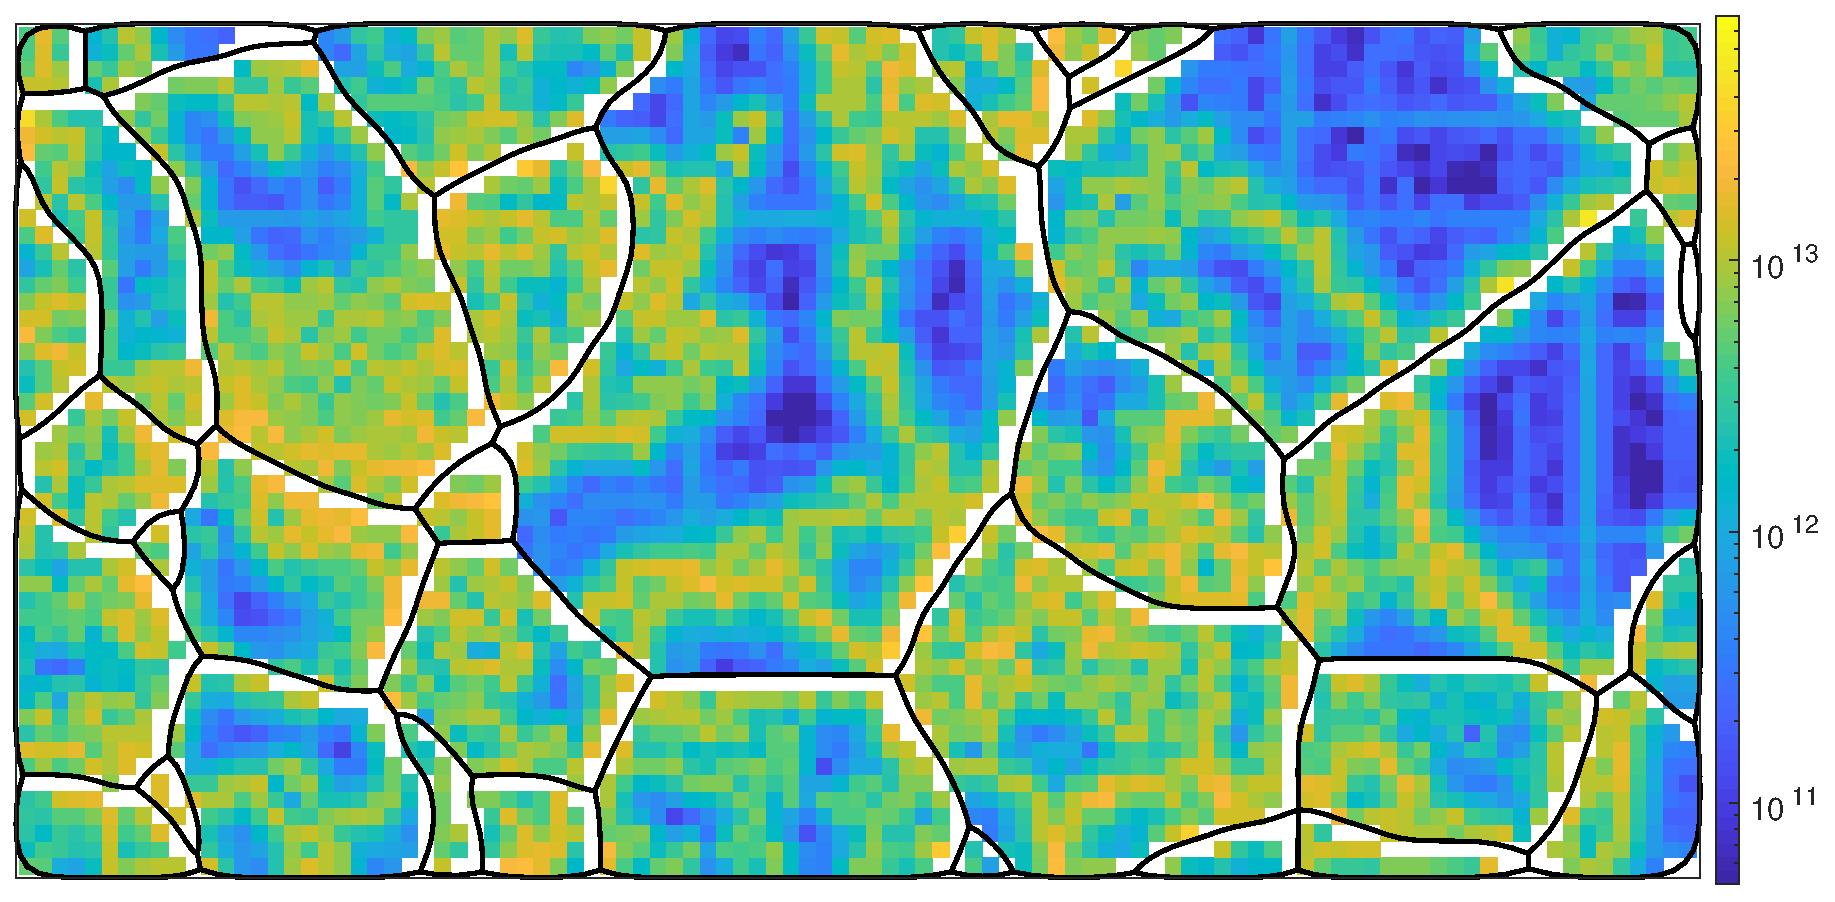
\includegraphics[width=0.93\textwidth]{pic/gnd.pdf}
  \end{center}
  \end{onlyenv}


\end{overlayarea}


% %% Soving the fitting problem
% % Now we are ready for fitting the dislocation tensors to the dislocation
% % densitiy tensor in each pixel of the map. This is done by the command
% % <curvatureTensor.fitDislocationSystems.html fitDislocationSystems>.

% [rho,factor] = fitDislocationSystems(kappa,dSRot);


\end{frame}

\end{document}
